\documentclass[12pt]{article}
\usepackage{amsmath,amssymb,amsthm}
\usepackage[english]{babel}
\usepackage[utf8]{inputenc}
\usepackage{fancyhdr}
\usepackage{changepage} 

\usepackage{hyperref}

% for line spacing
\usepackage{setspace}

% for absolute value
\usepackage{commath}

% for numbering
\usepackage{enumerate}

% for image placing
\usepackage{float}

% paper size and margins
\usepackage[letterpaper, left=20mm, right=20mm, top=25mm, bottom = 25mm, headsep=.15in]{geometry}

% code highlighting
\usepackage{minted}

% for curly brace
\usepackage{amsmath}

% for input images
\usepackage{graphicx}
\graphicspath{ {./} }
\usepackage{subfig}

% for printing pseudocode
\usepackage[boxed]{algorithm}
\usepackage[noend]{algpseudocode}

% for tables
\usepackage{tabularx}

\makeatletter
\def\BState{\State\hskip-\ALG@thistlm}
\makeatother

% for circled numbers
\usepackage{tikz}
\newcommand*\circled[1]{\tikz[baseline=(char.base)]{
            \node[shape=circle,draw,inner sep=1pt] (char) {#1};}}

% double line space
\renewcommand{\baselinestretch}{2.0}

% header, footer and page number
\pagestyle{fancy}
\fancyhf{}
\rhead{Tiankai Jiang \quad 20834939}
\lhead{ECE657A \quad Assignment 3}
\fancyfoot[C]{\thepage}

\setlength{\headheight}{15pt}

\begin{document}
\noindent
{\LARGE The source code is at the end of this document}
\section{Classification: Convolutional Neural Networks}

\subsection{Design and Implementation Choices of your Model}

Inspired by \href{https://arxiv.org/pdf/1409.1556.pdf}{VGG} and \href{https://arxiv.org/pdf/1512.03385.pdf}{ResNet}, almost all convolution layers are 3$\times$3 and almost all pooling layers are 2$\times$2.

The following CNN models are tested. 

\textbf{Model 1}

CNN1 is a sample CNN with only one convolutional layer. Dropout layer is used, which is the easiest way to prevent overfitting.
\begin{figure}[H]
\begin{center}
    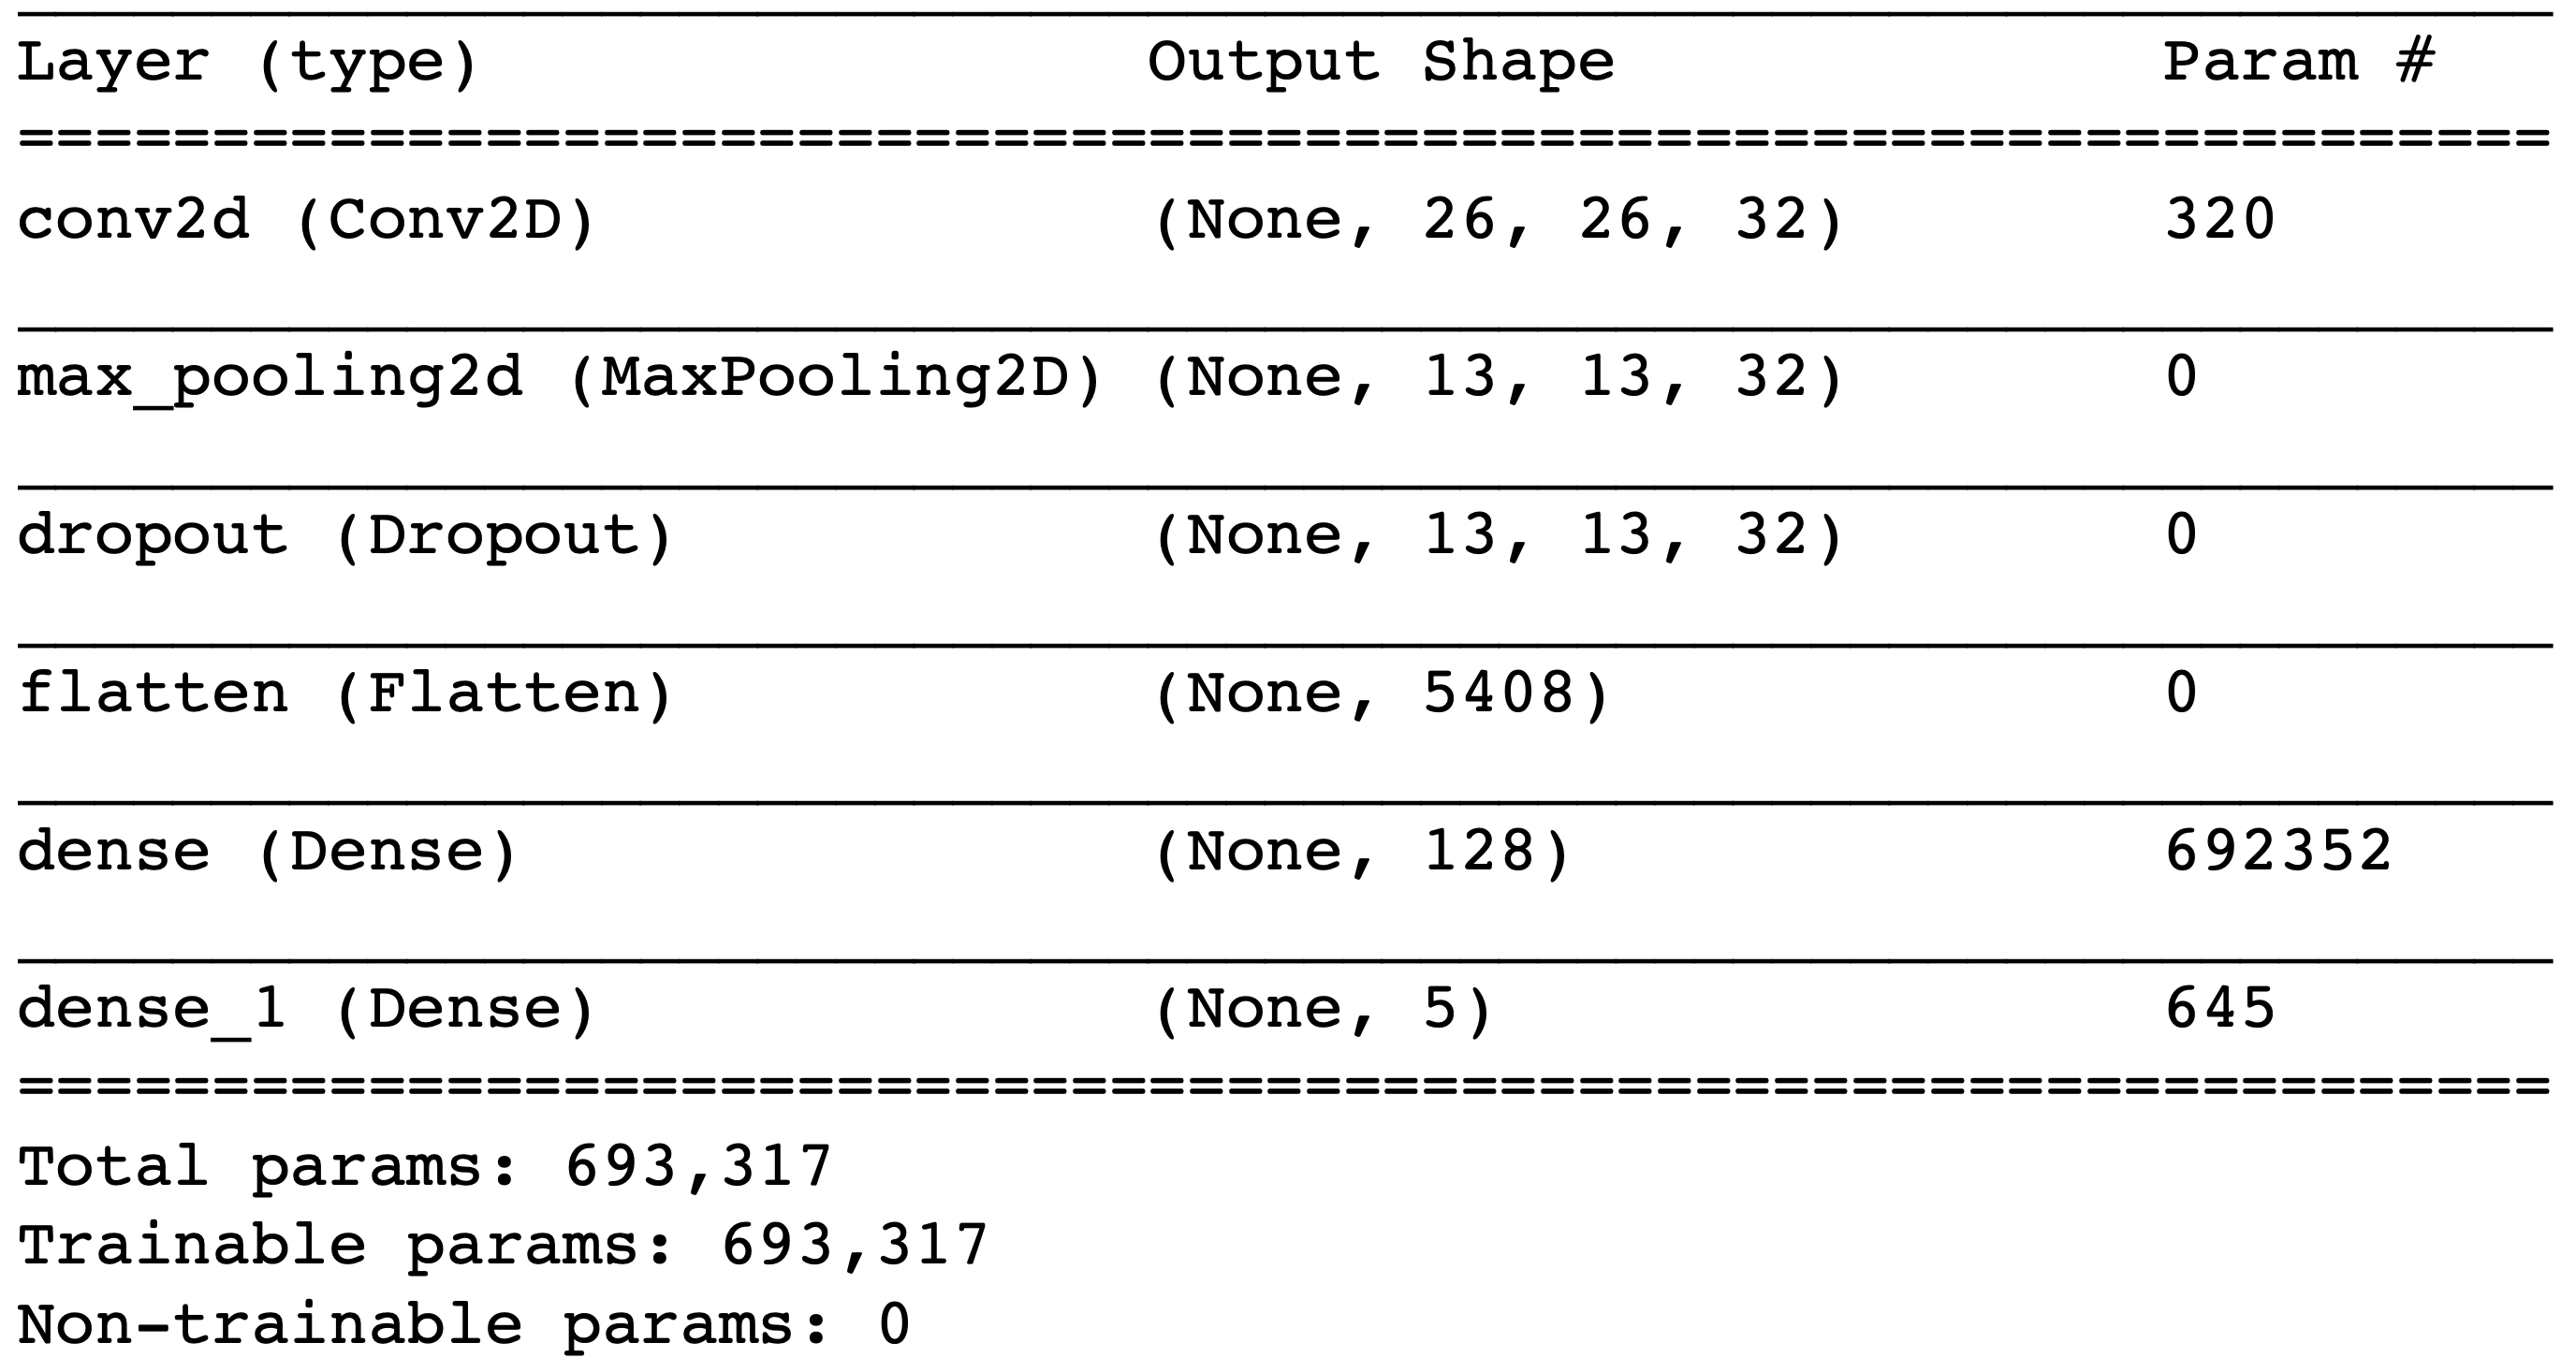
\includegraphics[width=1.0\textwidth]{./plots/1.png}
\end{center}
\end{figure}
\vspace*{-1.0cm}

\textbf{Model 2}

CNN2 is similar to the network in the \href{https://www.kaggle.com/fuzzywizard/fashion-mnist-cnn-keras-accuracy-93/}{link given in the assignment}. It has four convolutional layers, each followed by a batch normalization layer, which outputs the previous layer by substracting the batch mean and dividing it by batch standard deviation. Batch normalizatoin could speed up training and increase the stability of the network.
\begin{figure}[H]
\begin{center}
    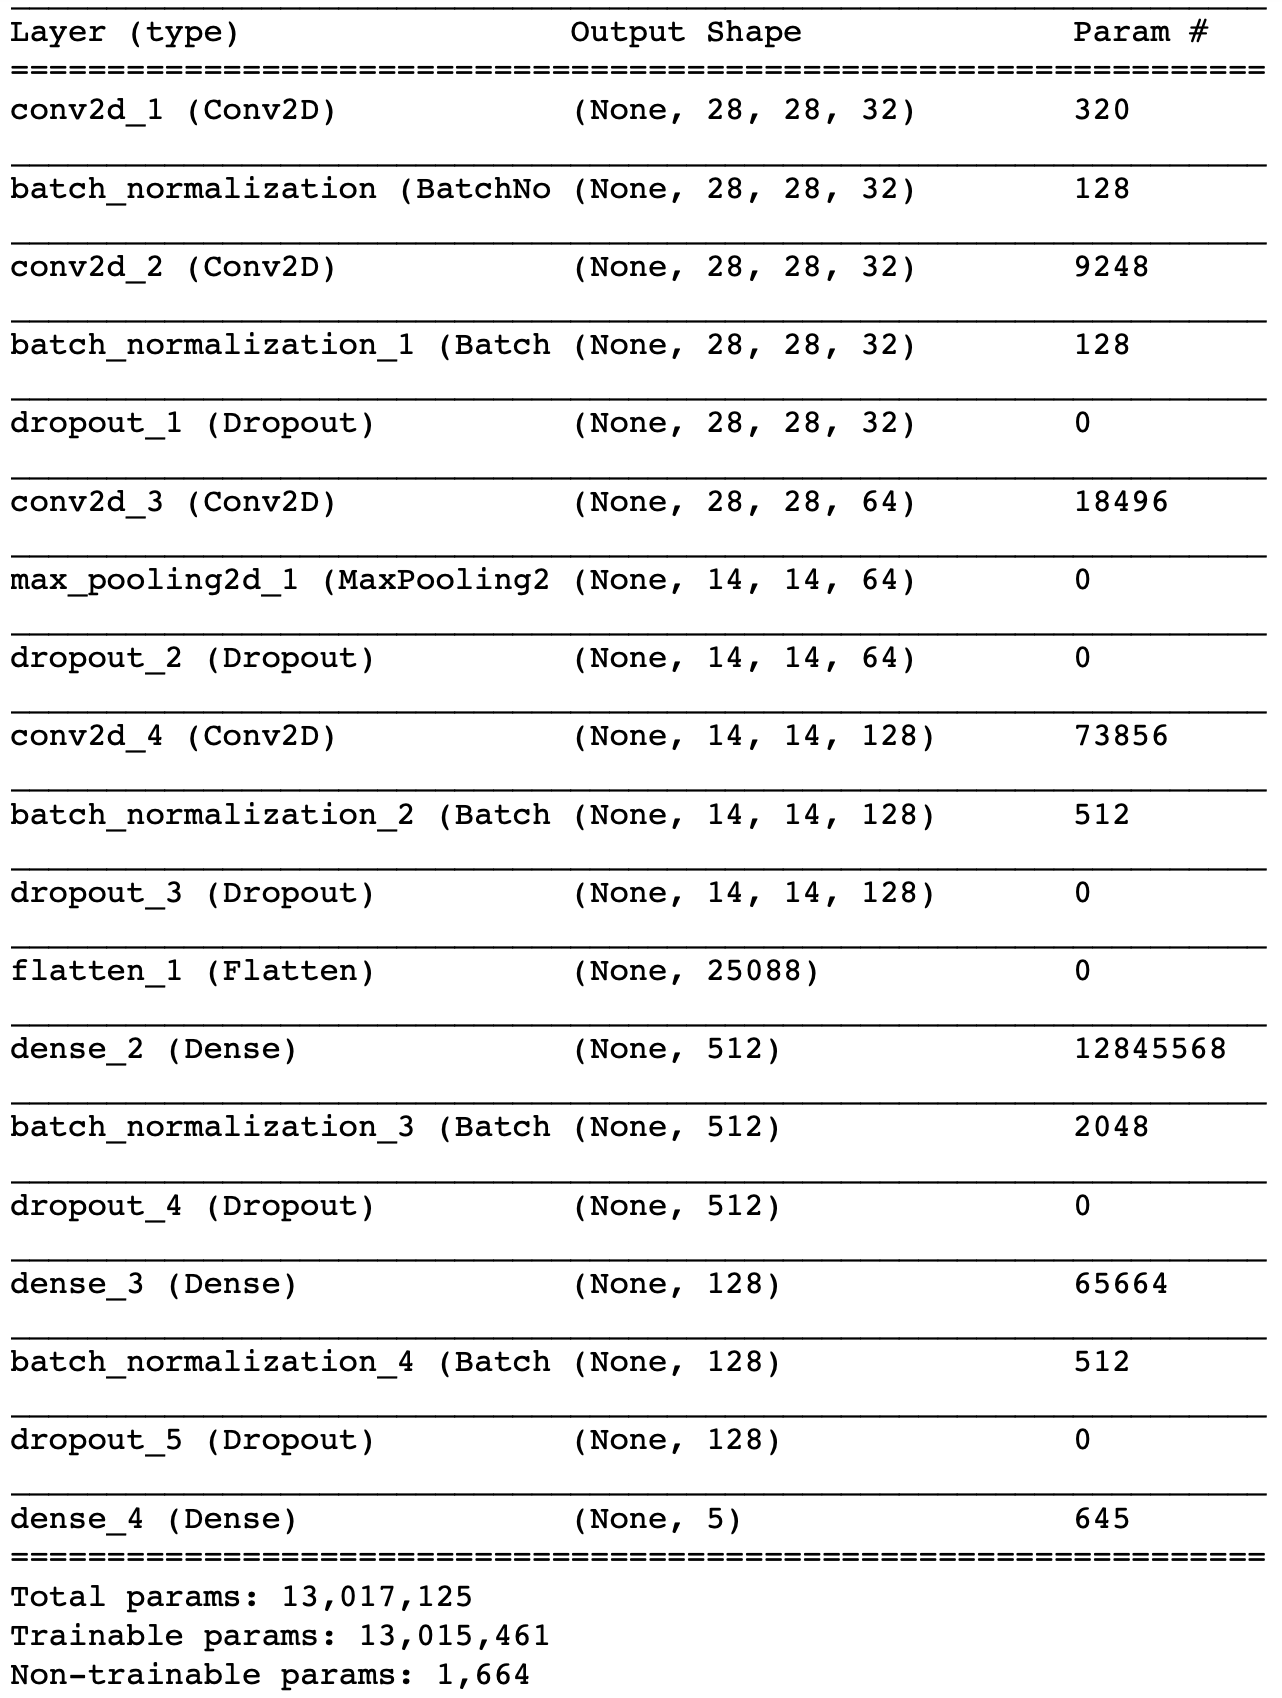
\includegraphics[width=0.83\textwidth]{./plots/2.png}
\end{center}
\end{figure}
\vspace*{-1.0cm}

\textbf{Model 3}

CNN3 is just CNN2 with an extra block(a Conv2D, a Batch normalization and a Dropout layer), because I wanted to check if a deeper network could do a better job.
\begin{figure}[H]
\begin{center}
    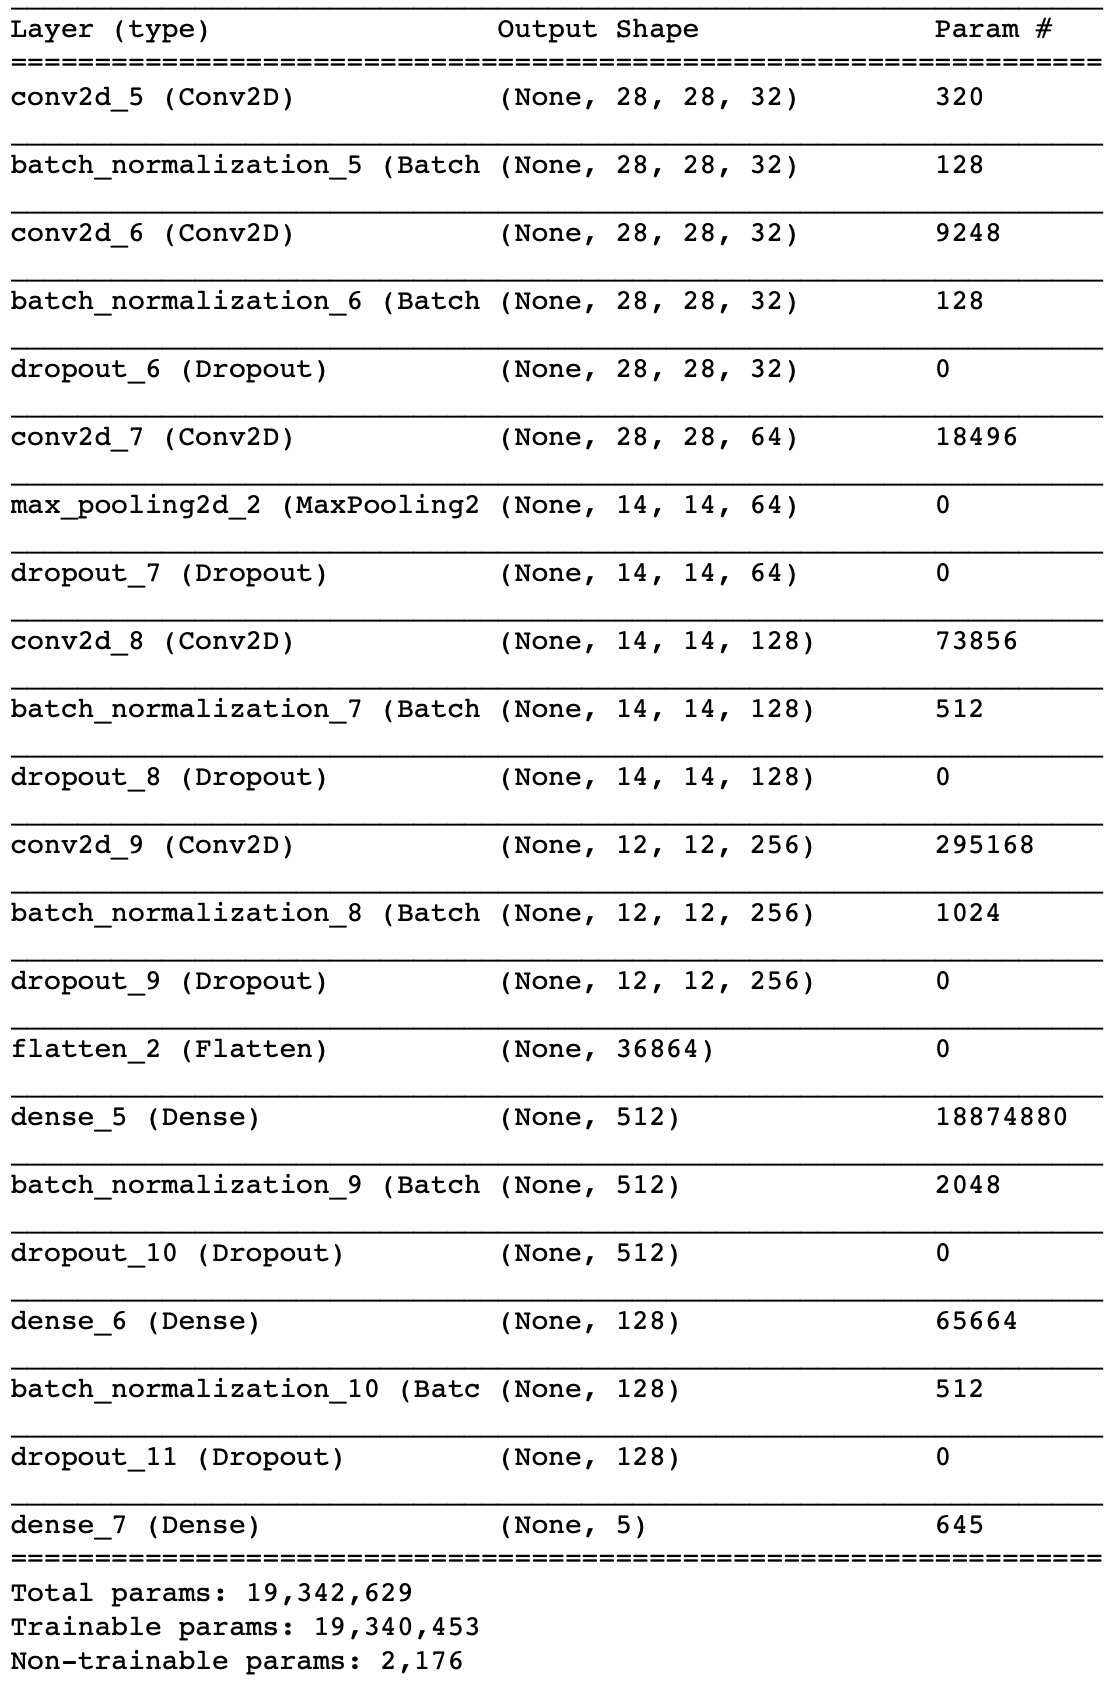
\includegraphics[width=0.73\textwidth]{./plots/3.png}
\end{center}
\end{figure}
\vspace*{-1.0cm}

\textbf{Model 4}

CNN4 is a VGG like network (two or three Convolutional layers followed by a pooling layer) given in \href{http://proc-x.com/2017/09/a-vgg-like-cnn-for-fashion-mnist-with-94-accuracy/}{this link}. Batch normalizatoin layer was also applied to speed up computation.
\begin{figure}[H]
\begin{center}
    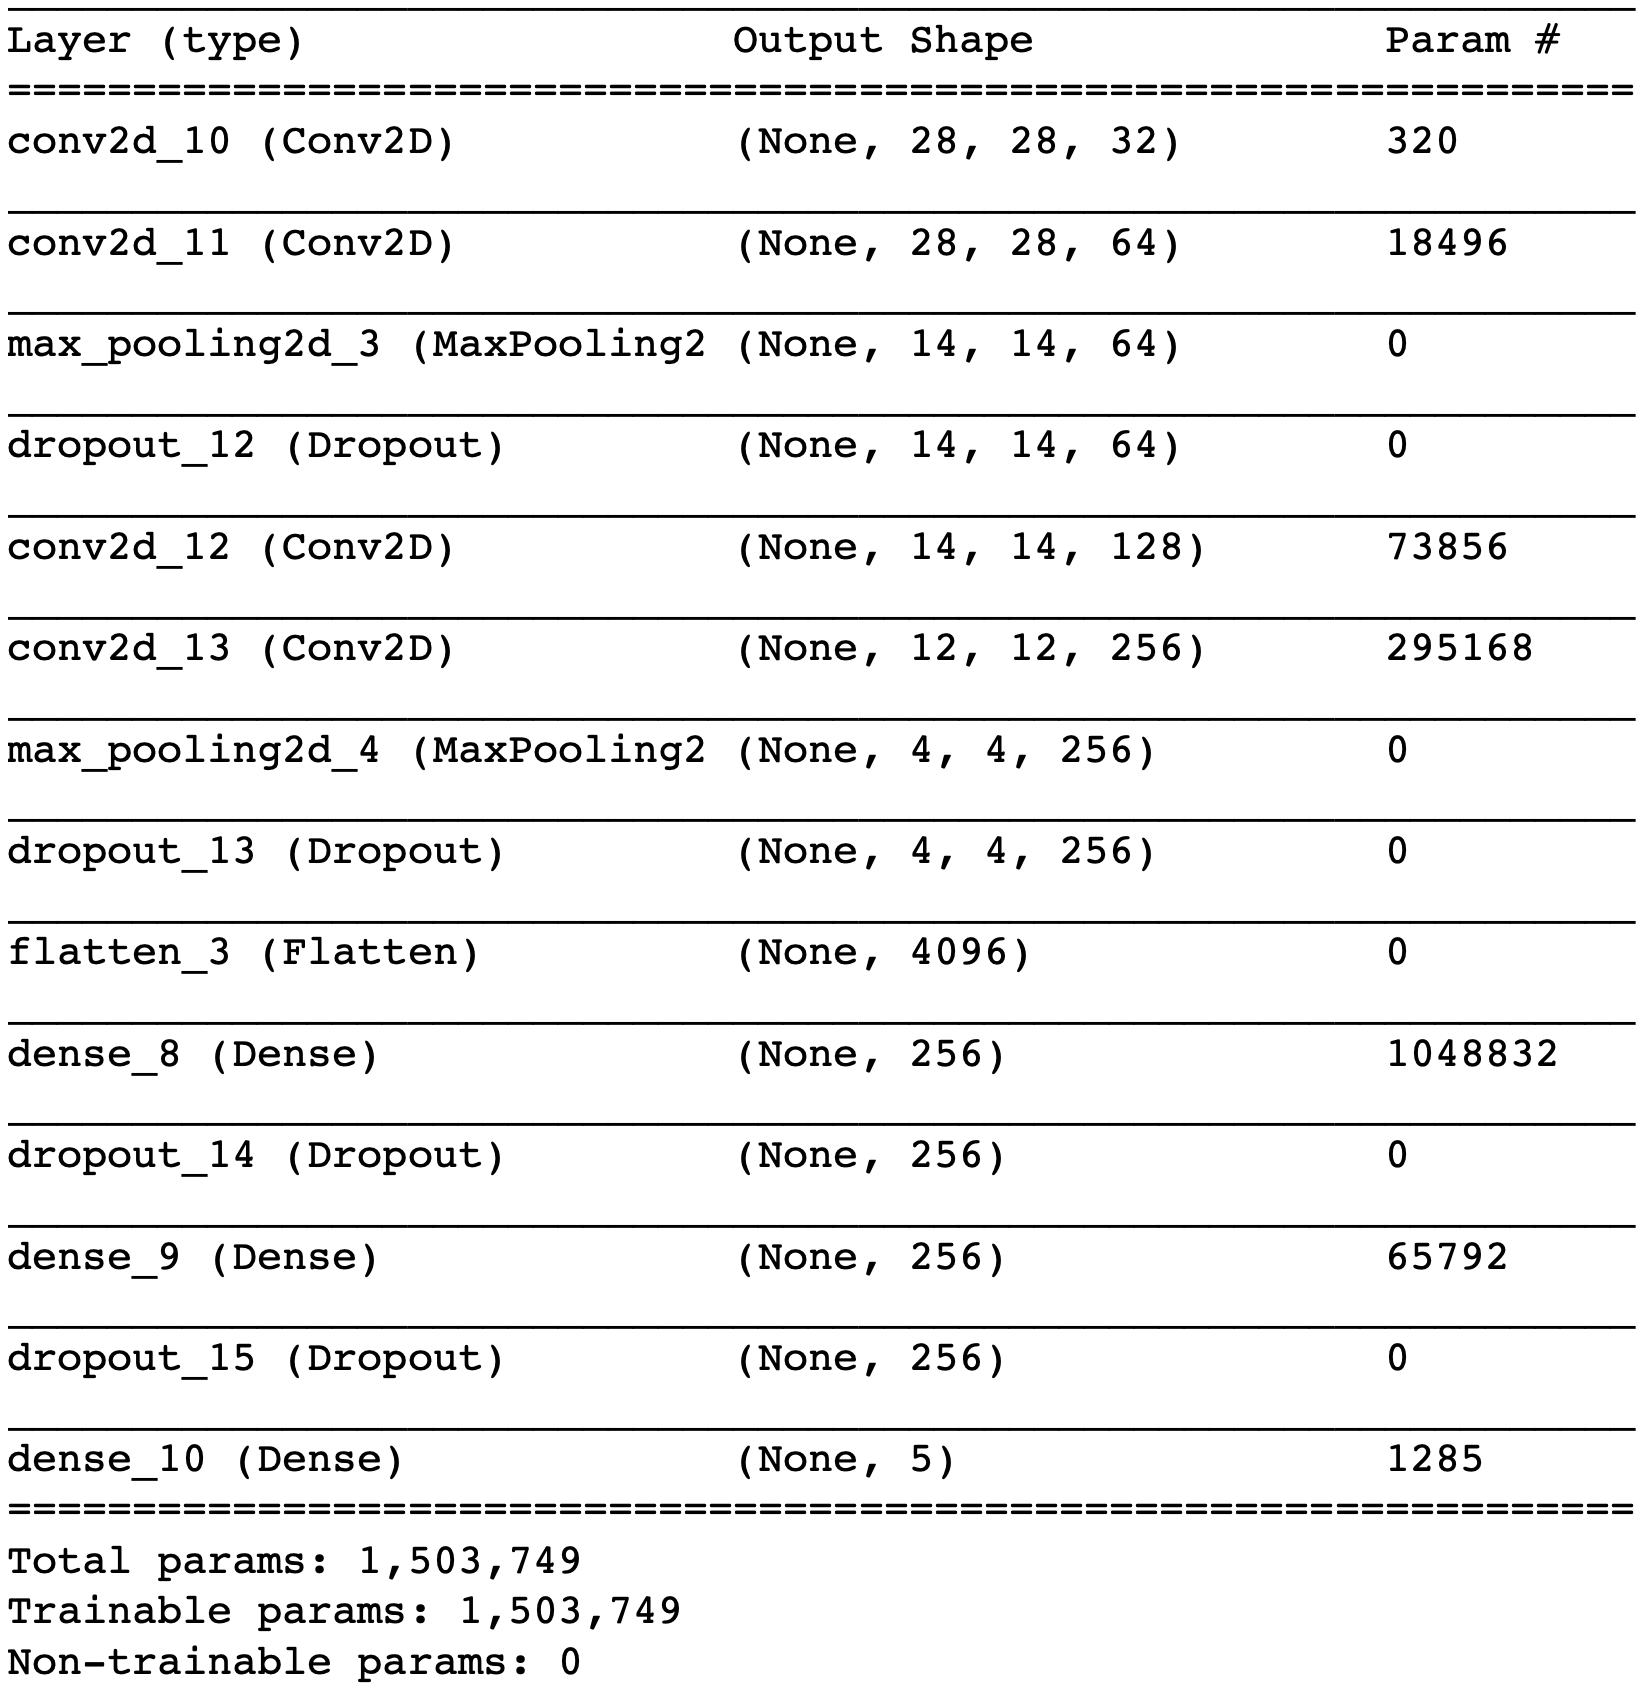
\includegraphics[width=0.8\textwidth]{./plots/4.png}
\end{center}
\end{figure}
\vspace*{-1.0cm}

\textbf{VGG19}

\href{https://arxiv.org/pdf/1409.1556.pdf}{VGG19} with imagenet pretrained weight. VGG19 contains 16 convolutional layers and 3 fully connected layers. VGG has a relatively simple network structure and it performs well in the image classification. Before using this model, I had to transform the input data into desired form. The origin input format of VGG19 is 224$\times$224$\times$3, and the minimum input dimension for keras VGG19 model is 32$\times$32$\times$3. I stacked the data three times and reshaped it to 150$\times$150, because a too small input would affect the performance of the network and 150$\times$150 is almost the largest size I could get within my computer's capability.

Its performance was really bad(accuracy 65.53\%) so I gave it up. Maybe because our labels were twisted and it was not a conventional image classification problem so we should not use the weights directly. 

\textbf{Inception V3}

Inception network stacks the result of multiple filters together, therefore, the network can learn small details, middle sized features and almost whole images at the same time. So it will usually achieve a good result.

Since using the pretrained weight directly was not a good idea, I tried transfer learning on Inception V3. We had to adjust the input format to 150$\times$150$\times$3 like VGG19, and last 10 layers of the model were retrained. 

The performance was bad as well(accuracy 40.03\%), so I did not try any further improvements.

\textbf{Inception}

The Inception V3 model is too big for us to train from scratch. Following \href{https://machinelearningmastery.com/how-to-implement-major-architecture-innovations-for-convolutional-neural-networks/}{this blog}, I built a smaller Inception network. But its accuracy was only 81.12\%. 
\begin{figure}[H]
\begin{center}
    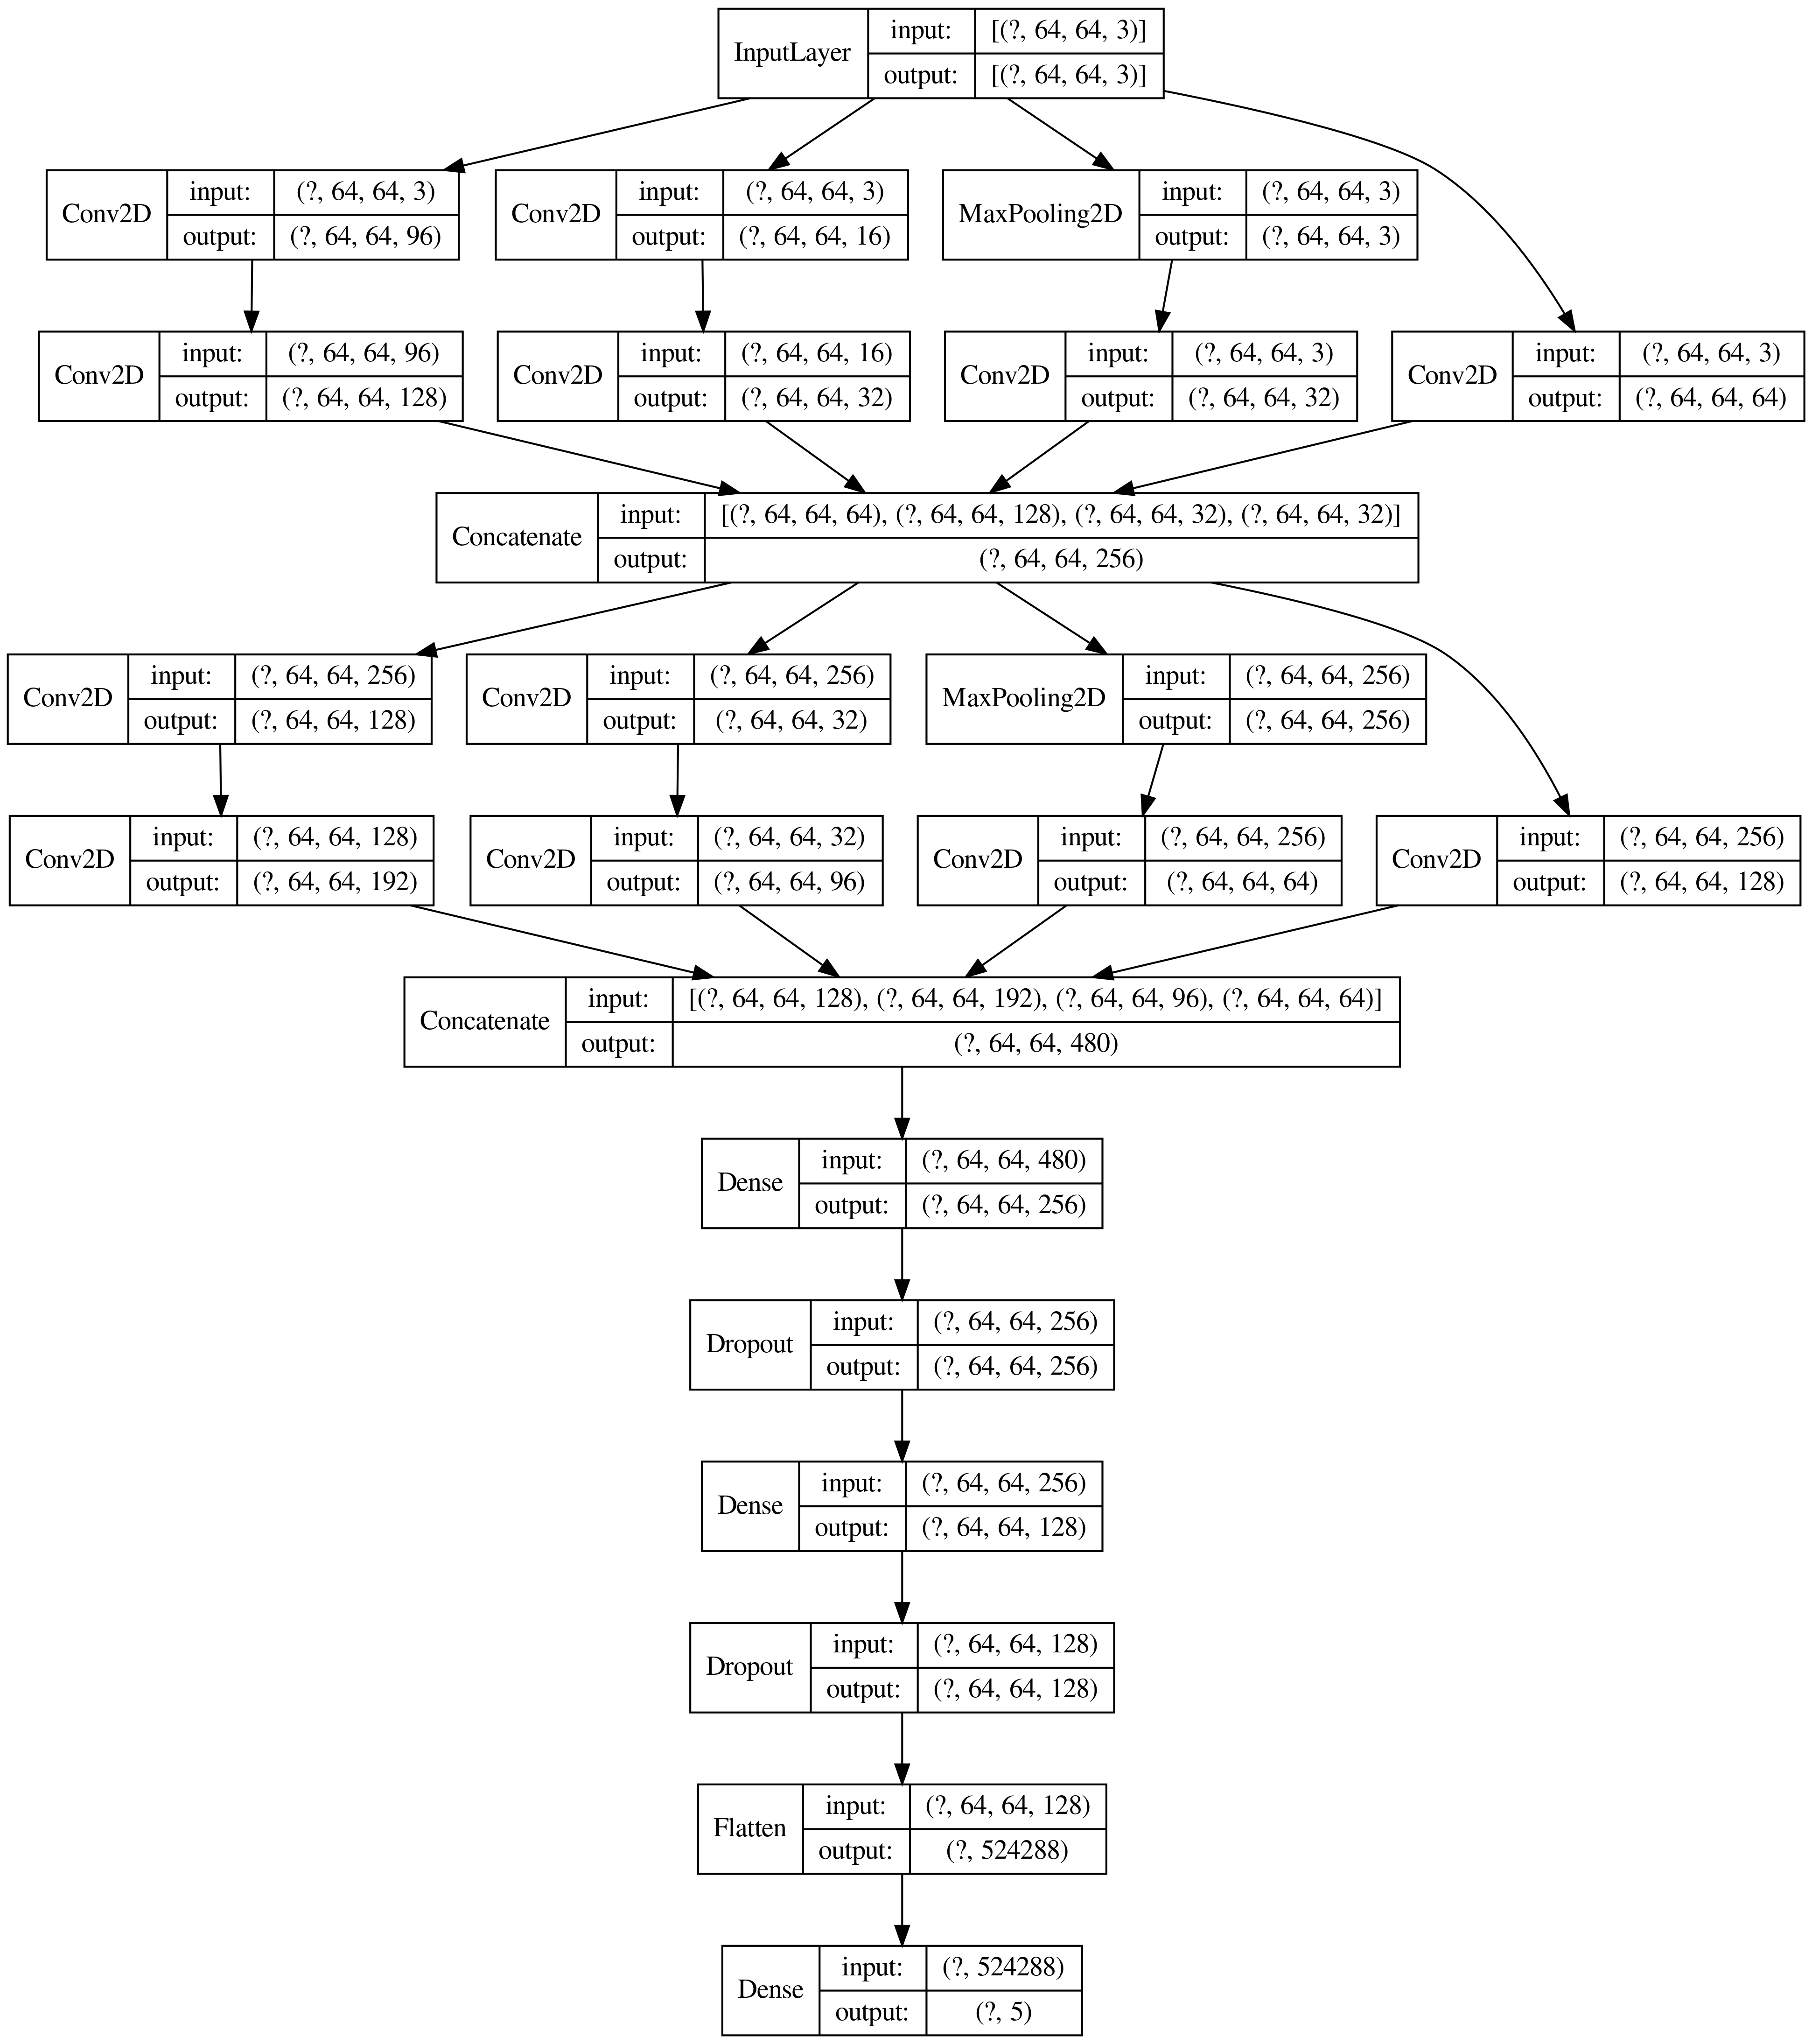
\includegraphics[width=1.0\textwidth]{./plots/Inception.png}
\end{center}
\end{figure}
\vspace*{-1.0cm}

\textbf{Resnet50}

When the network becomes deeper and deeper, the model is prone to overfitting the data. Also, when performing the back-propagation, the gradient may becomes infinitively small or really big, making it harder to make progress. By skipping one or more layers, that is connecting one layer directly to a layer several depth apart, the model becomes more robust. This shortcut connection makes it possible for us to build deeper networks.

The Resnet50 used here was implemented based on \href{https://www.coursera.org/learn/convolutional-neural-networks?specialization=deep-learning#syllabus}{Coursera CNN week 2 programming assignments}.

The whole structure is too large to show. Only part of it is shown below. The left one is convolutional block and the right one is identity block. Resnet50 is basically the stacking of these two blocks.
\begin{figure}[H]
\captionsetup[subfigure]{labelformat=empty}
\centering
\subfloat[]{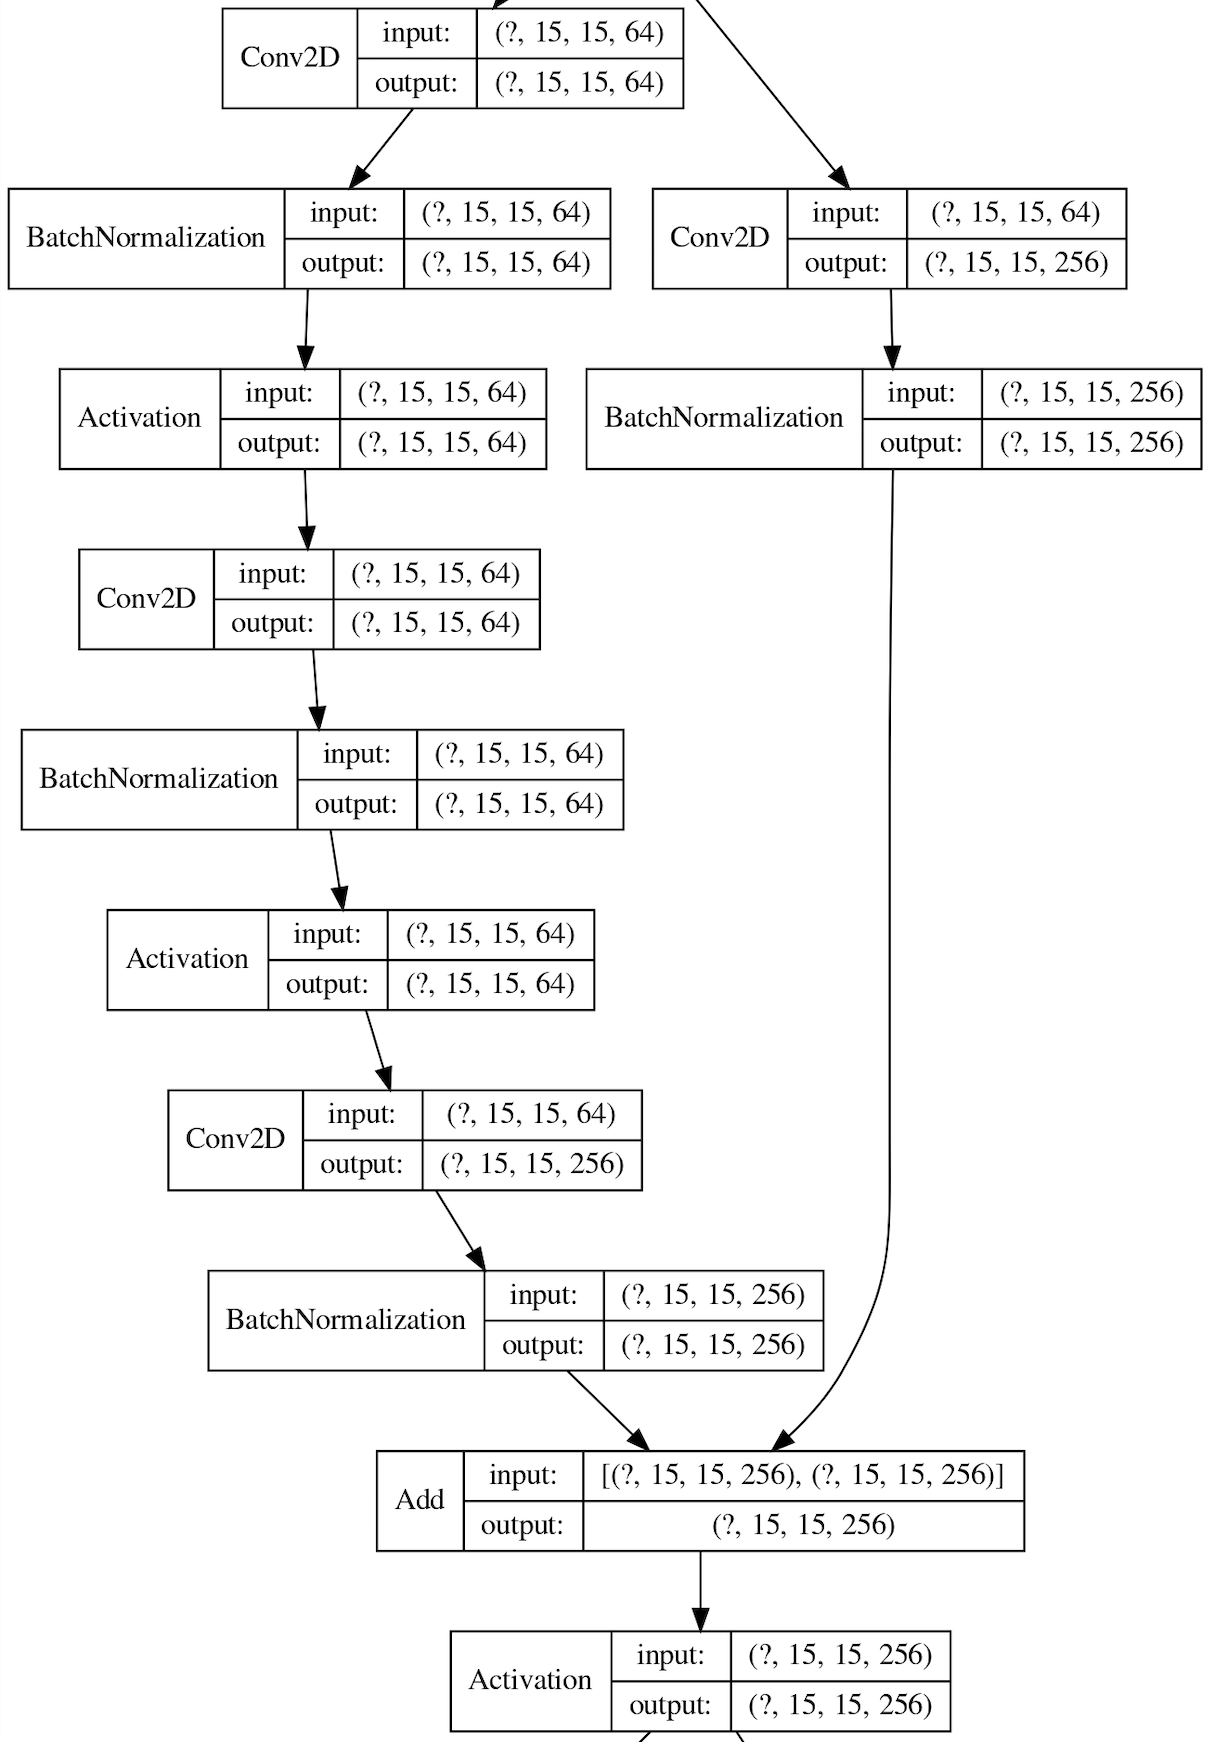
\includegraphics[width=0.5\textwidth]{./plots/ResNet50_1.png}}
\subfloat[] {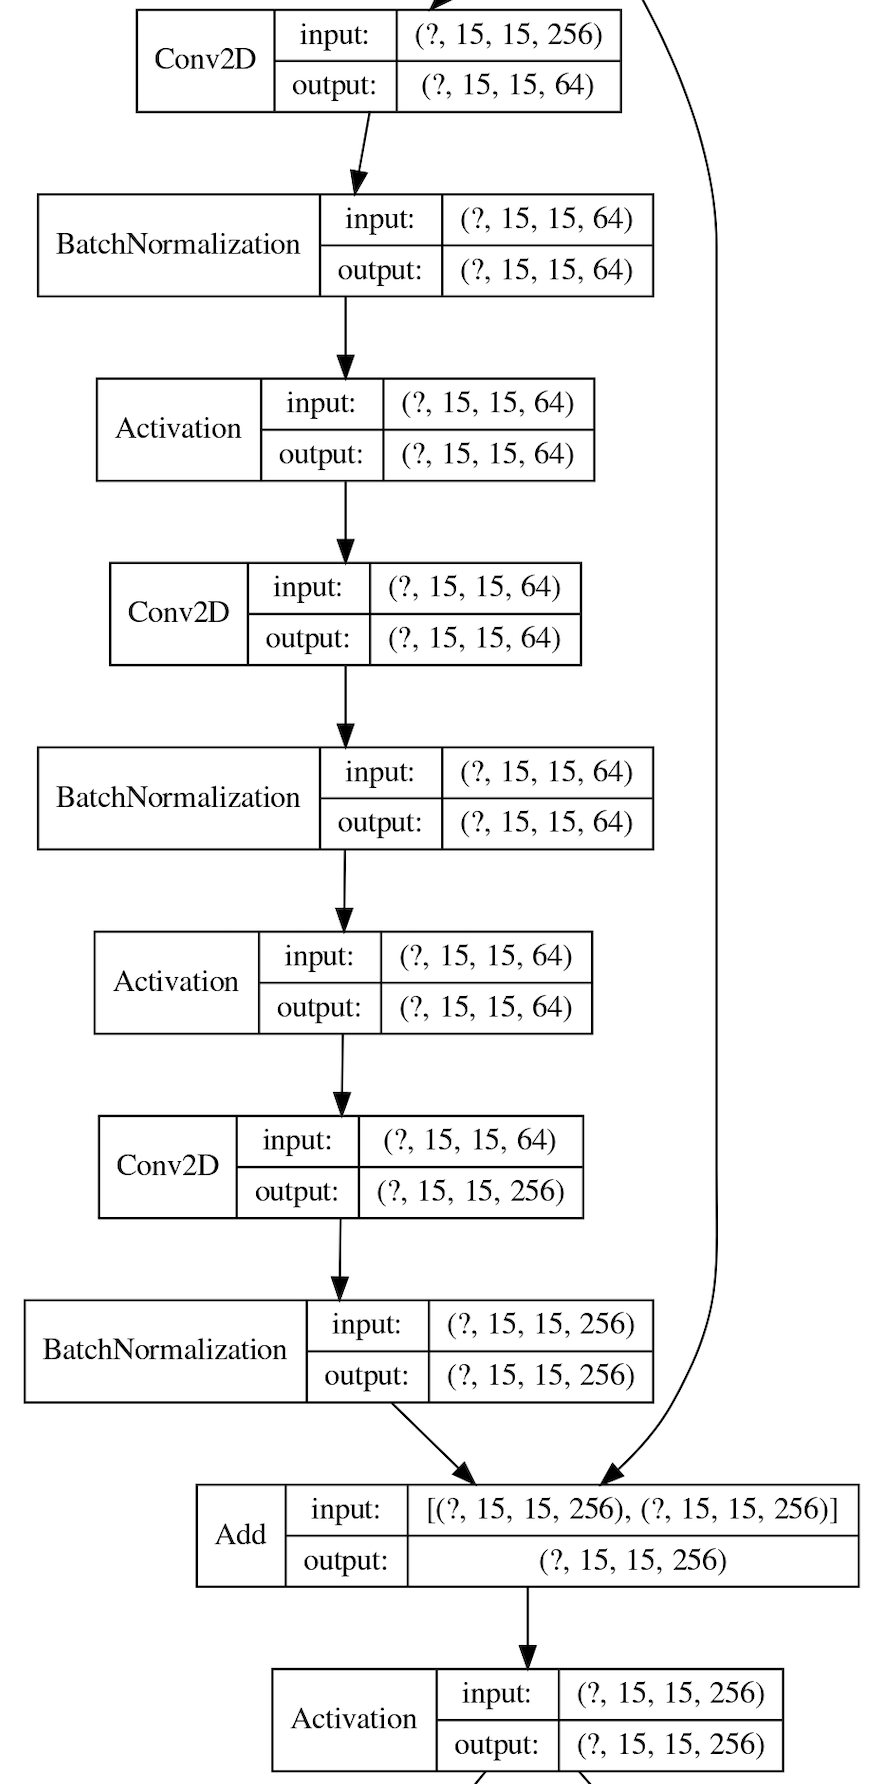
\includegraphics[width=0.38\textwidth]{./plots/ResNet50_2.png}}
\end{figure}

\textbf{Data Augmentation}

ImageDataGenerator was used to generate transformed images for neural networks. Each image was zoomed, rotated, flipped or sheared and then fed to the network. But it did not perform well as expected. The validation accuracy decreased gradually from around 90 percent to 82 percent as more and more data being generated. Hence, data augmentation was not used later.\\

Hyperparameters, regularization and optimizers will be discussed later.

\subsection{Implementation of your Design Choices}

\begin{singlespacing}
\begin{itemize}
\item A sequential model(take model 1 as example)
\begin{minted}[linenos,tabsize=4,breaklines]{python}
CNN1 = Sequential([
    Conv2D(filters=32, kernel_size=(3, 3), activation='relu', input_shape=(28,28,1)),
    MaxPool2D(pool_size=(2, 2)),
    Dropout(0.5),
    Flatten(),
    Dense(128, activation='relu'),
    Dense(5, activation='softmax')
])
CNN1.compile(optimizer='adam', loss="categorical_crossentropy", metrics=["accuracy"])
historyCNN1 = CNN1.fit(X_train, y_train, epochs = 30, batch_size=128, validation_data = (X_val, y_val))
\end{minted}

\item Data augmentation
\begin{minted}[linenos,tabsize=4,breaklines]{python}
datagen = ImageDataGenerator(rotation_range = 8, zoom_range = 0.1, shear_range = 0.3, width_shift_range=0.08, height_shift_range=0.08, vertical_flip=True)
history = model.fit(datagen.flow(X_train, y_train, batch_size = 128), epochs = 40, validation_data = (X_test, y_test), steps_per_epoch=X_train.shape[0] // 128, callbacks = [reduce_lr])
\end{minted}

\item Class to record training and testing time in one epoch
\begin{minted}[linenos,tabsize=4,breaklines]{python}
class TimeHistory(Callback):
    def on_train_begin(self, logs={}):
        self.times = []

    def on_epoch_begin(self, batch, logs={}):
        self.epoch_time_start = time()

    def on_epoch_end(self, batch, logs={}):
        self.times.append(time() - self.epoch_time_start)
\end{minted}

\item Use pretrained weight
\begin{minted}[linenos,tabsize=4,breaklines]{python}
vgg19 = VGG19(weights='imagenet', include_top=False, input_shape = (150, 150, 3), classes = 5)
X_train = keras.applications.vgg19.preprocess_input(X_train)
train_features = vgg19.predict(np.array(X_train), batch_size=256)
train_features = np.reshape(train_features, (48000, 4*4*512))
# then put the trained features to a single layer network to produce output
\end{minted}

\item Accuracy and loss plot
\begin{minted}[linenos,tabsize=4,breaklines]{python}
def acc_plot(history, name):
    plt.figure(figsize=(10,6))
    plt.plot(history['accuracy'], label='training accuracy')
    plt.plot(history['loss'], label='training loss')    
    plt.plot(history['val_accuracy'], label='validation accuracy')
    plt.plot(history['val_loss'], label='validation loss')
    plt.title(name + ' Accuracy and Loss')
    plt.xlabel('epochs')
    plt.legend()
    return plt.show()
\end{minted}

\item The code to create non-sequential models like Inception and Resnet50 and the code for transfer learning are too long to put it here, please check the source code.
\end{itemize}
\end{singlespacing}

\subsection{Kaggle Competition Score}

0.92240

Achieved using ensemble method. Train Model 1 repeatedly and only keep the predicted result if its testing accuracy is greater than 91 percent. Collect about 30 predicted results and vote like random forest. It took around 36 hours to get 30 qualified results using a single GTX 1080 Ti.

\subsection{Results Analysis}

\subsubsection{Runtime performance for training and testing}

The training and predicting time \textbf{for one epoch} for each method is shown below:
\begin{center}
\begin{tabular}{|p{2.5cm}|p{2.5cm}|p{2.5cm}|}
\hline
\textbf{Model} & \textbf{Training(s)} & \textbf{Testing(s)}\\ 
\hline
1(3 layers) & 1.84 & 1.21\\ 
\hline
2(7 layers) & 5.92 & 1.84\\ 
\hline
3(8 layers) & 8.01 & 1.88\\ 
\hline
4(7 layers) & 4.68 & 1.43\\
\hline
Inception & 161.96 & 14.30\\
\hline
Resnet50 & 36.01 & 7.66\\
\hline
\end{tabular}
\end{center}

For sequential models, the more parameters to train, the slower it will get. But the number of parameters and training time does not grow proportionally. Model 2 has 19,340,453 trainable params and model 4 has 1,503,749, yet their training time for one epoch are similar, which indicates that the structure of the network also affects run time. Inception has only 3,290,597 trainable params, however, it takes way longer to train. Resnet50 has 23,544,837 trainable params but it is 3.5 times faster than Inception.

\subsubsection{Comparison of the different algorithms and parameters you tried}
\begin{center}
\begin{tabularx}{0.8\textwidth} { 
| >{\raggedright\arraybackslash}X 
| >{\raggedleft\arraybackslash}X | }
\hline
\textbf{Model} & \textbf{Accuracy}\\ 
\hline
1(3 layers) & 79.10\%-91.36\%\\ 
\hline
2(7 layers) & 85.68\%-90.15\%\\ 
\hline
3(8 layers) & 87.42\%-90.47\%\\ 
\hline
4(7 layers) & 89.68\%-90.15\%\\
\hline
Inception & 81.12\%\\
\hline
Resnet50 & 88.77\%-89.56\%\\
\hline
\end{tabularx}
\end{center}

As we can see from the table, generally, the deeper a network, the more stable its performance. Model 1 only has 3 layers and its accuracy on validation set fluctuate a lot. 79.10\% and 91.36\% are both very rare cases, they occur only once or twice in hundreds of runs. The accuracy is about 88\% on average. Also, we cannot say that model 1 is better than others because its best performance is 91.36\%. Because it is the easiest to train(it took only 3s to train a batch with batchsize = 128), I could train it hundreds of times but for other models, it takes tens of minutes to hours to train. So I could only train them a few times. Model 2 and 4 are both 7 layers but model 4 is more stable than model 2. This may due to its VGG like structure.

The performance of Inception and Resnet50 are disappointing. It took 10 times longer to train them but the accuracy is worse than a simple VGG like model. A possible explanation for this is that the training set is not large enough. For the original Inception and Resnet, they are trained by millions of 
224$\times$224 colored images. However, we only have 60,000 28$\times$28 grey scale images. The lack of input information made it difficult to build an accurate model.

\subsubsection{Explanation of your model}

The structure of each model have been shown in section 1.1. This section will mainly focus on hyperparameters, regularization and optimizers.

ReduceLROnPlateau was used as callback function on every model to reduce learning rate when the accuracy has stopped improving.

Only dropout layer as regularisation was used because it is the easiest one.

The epochs was set as 40 initially and later I would check if there was sign of overfitting. If there was, the number would be decreased.

The batch size was set as 128 or 256. These two numbers led to similar performance.

Activation function: softmax for output layer and ReLU for others.

The following hyperparameters are tuned using hyperas and hyperopt following \href{https://towardsdatascience.com/a-guide-to-an-efficient-way-to-build-neural-network-architectures-part-ii-hyper-parameter-42efca01e5d7}{this guide}:
\begin{itemize}
  \item Dropout rate: a random number between 0 and 1.
  \item Number of units in a Dense layer: 128, 256 or 512.
  \item Optimizer: Adam, SGD or RMSProp, each with learning rate of 0.001, 0.01 or 0.1.
\end{itemize}

However, I found hyperas not so efficient and sometimes it generated a set of parameters that led to a really mediocre result after 30-50 evaluation.

\subsubsection{Plots}
Loss, Accuracy vs Epochs for each model(except for Inception because it has only 82\% accuracy) are plotted.
\begin{figure}[H]
\begin{center}
    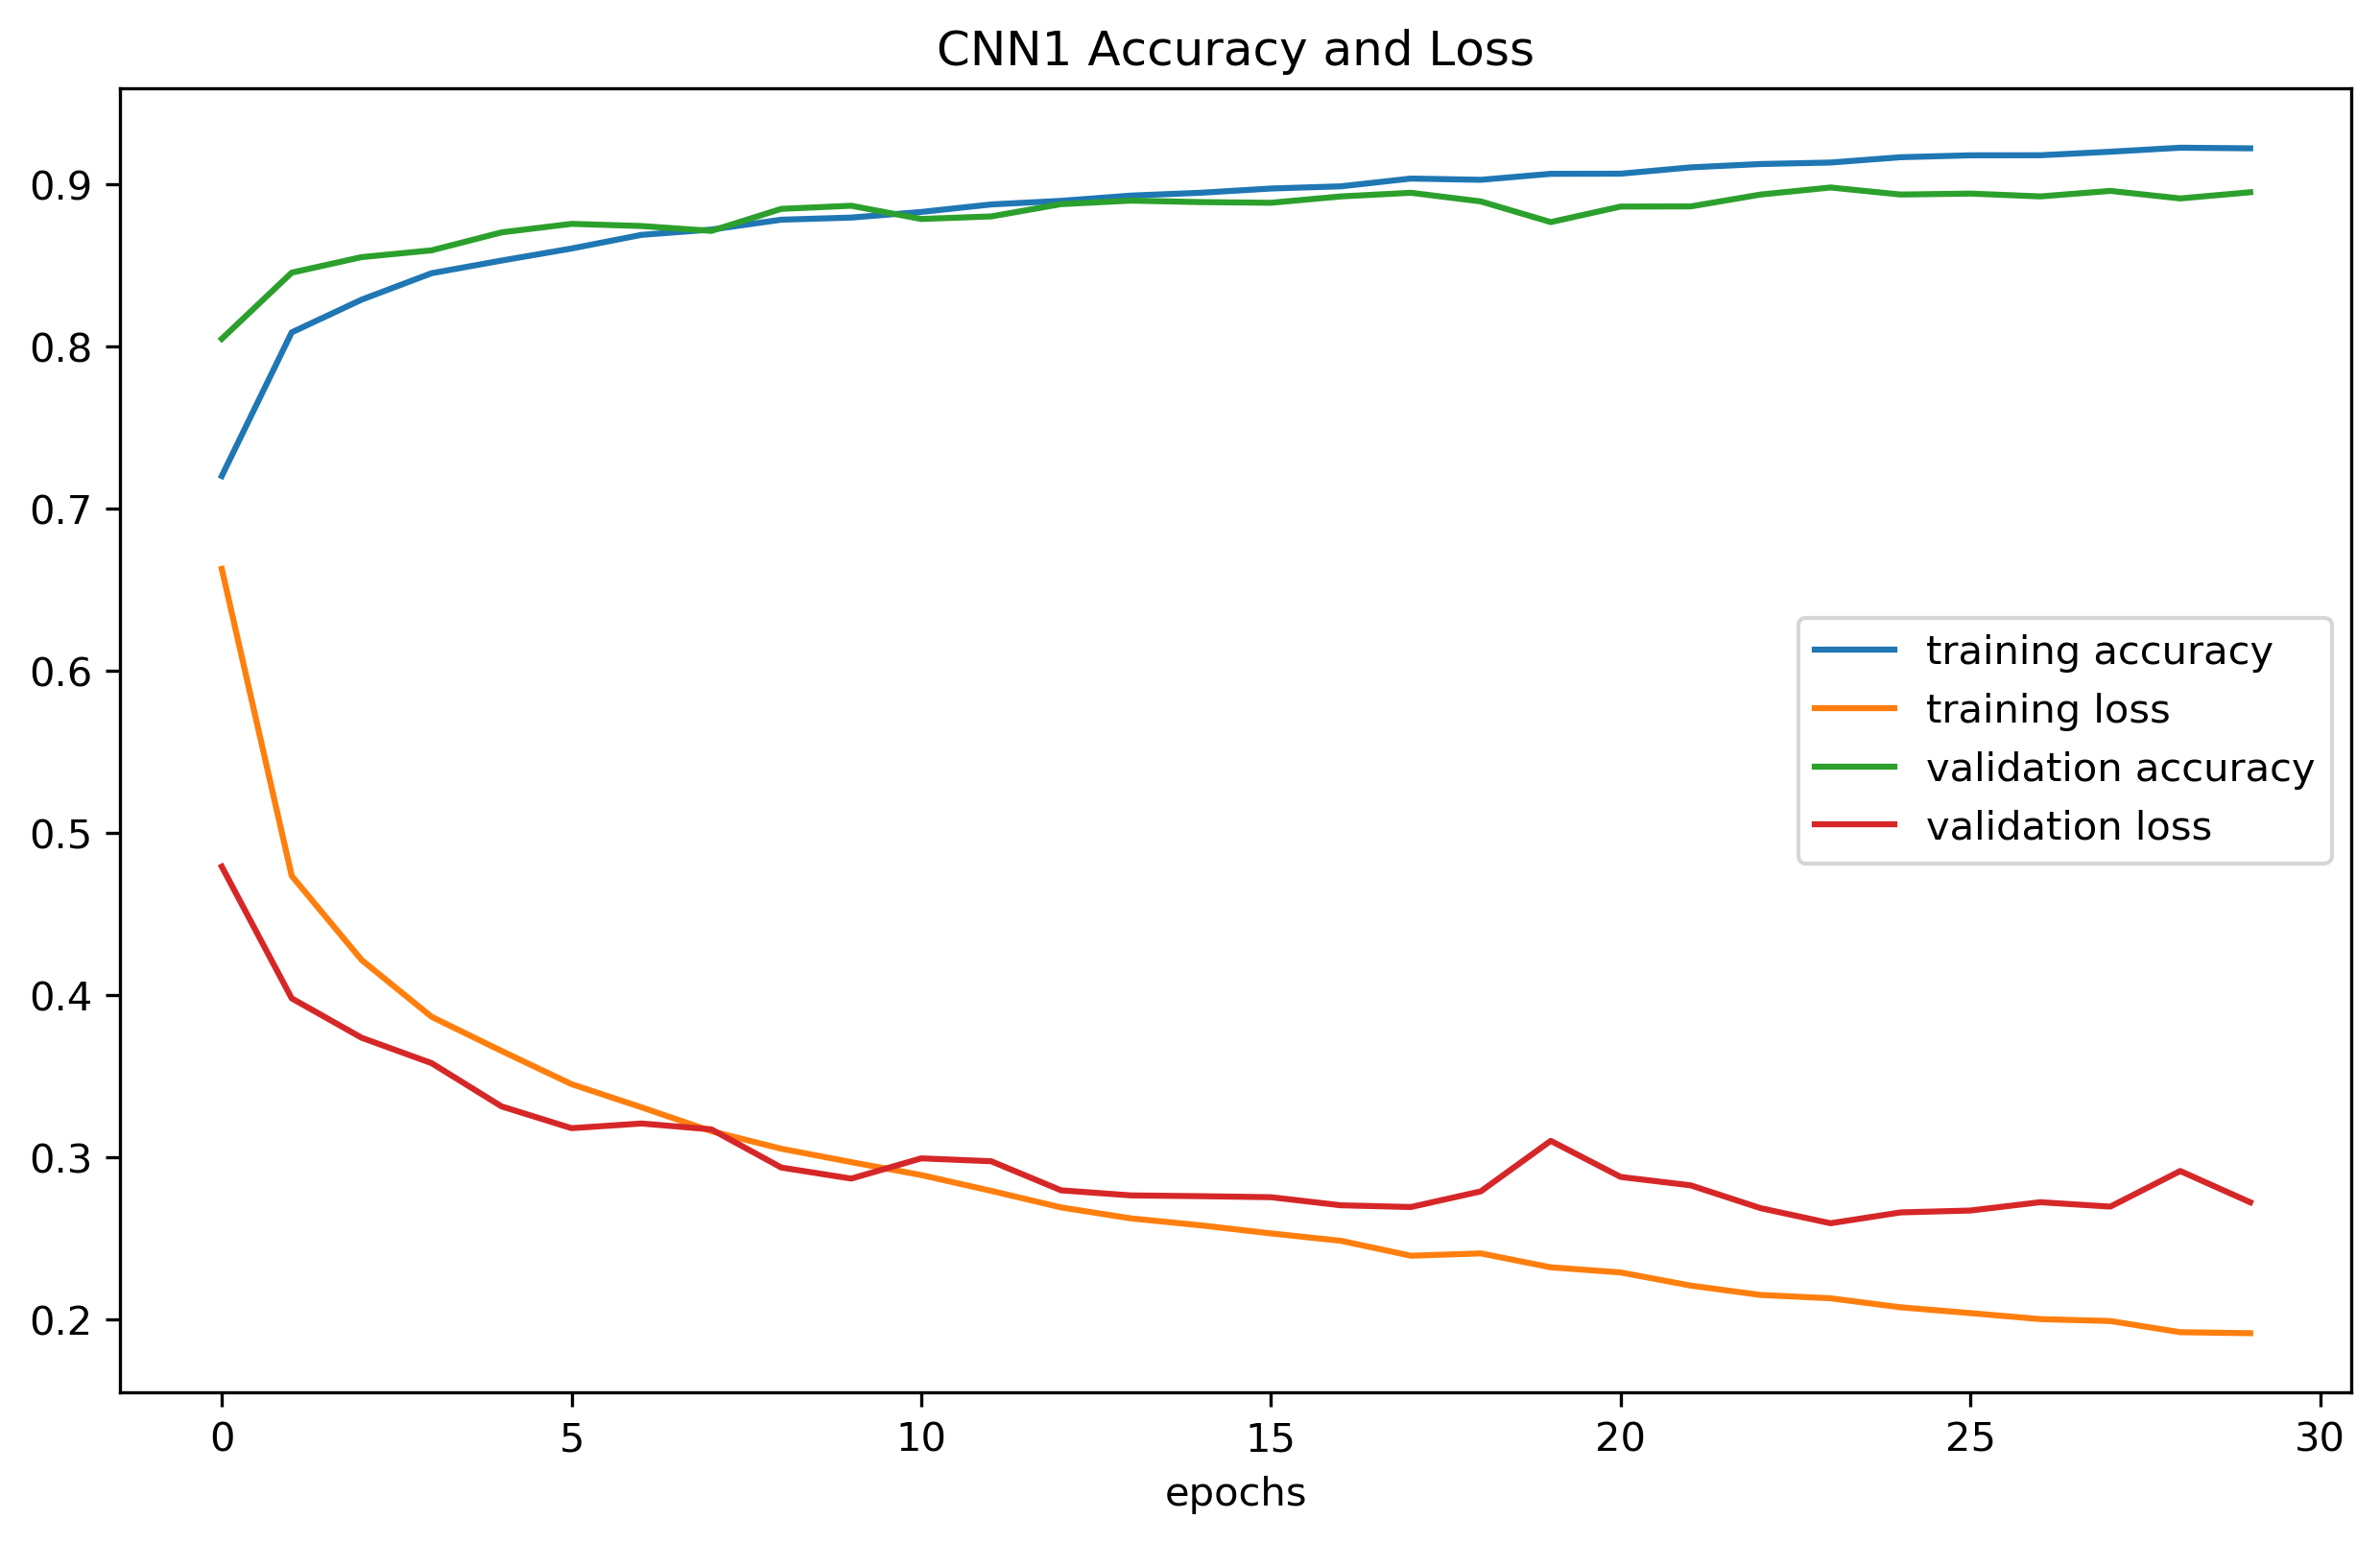
\includegraphics[width=0.8\textwidth]{./plots/CNN1_Result.png}
\end{center}
\end{figure}
% \vspace*{-1.5cm}
\begin{figure}[H]
\begin{center}
    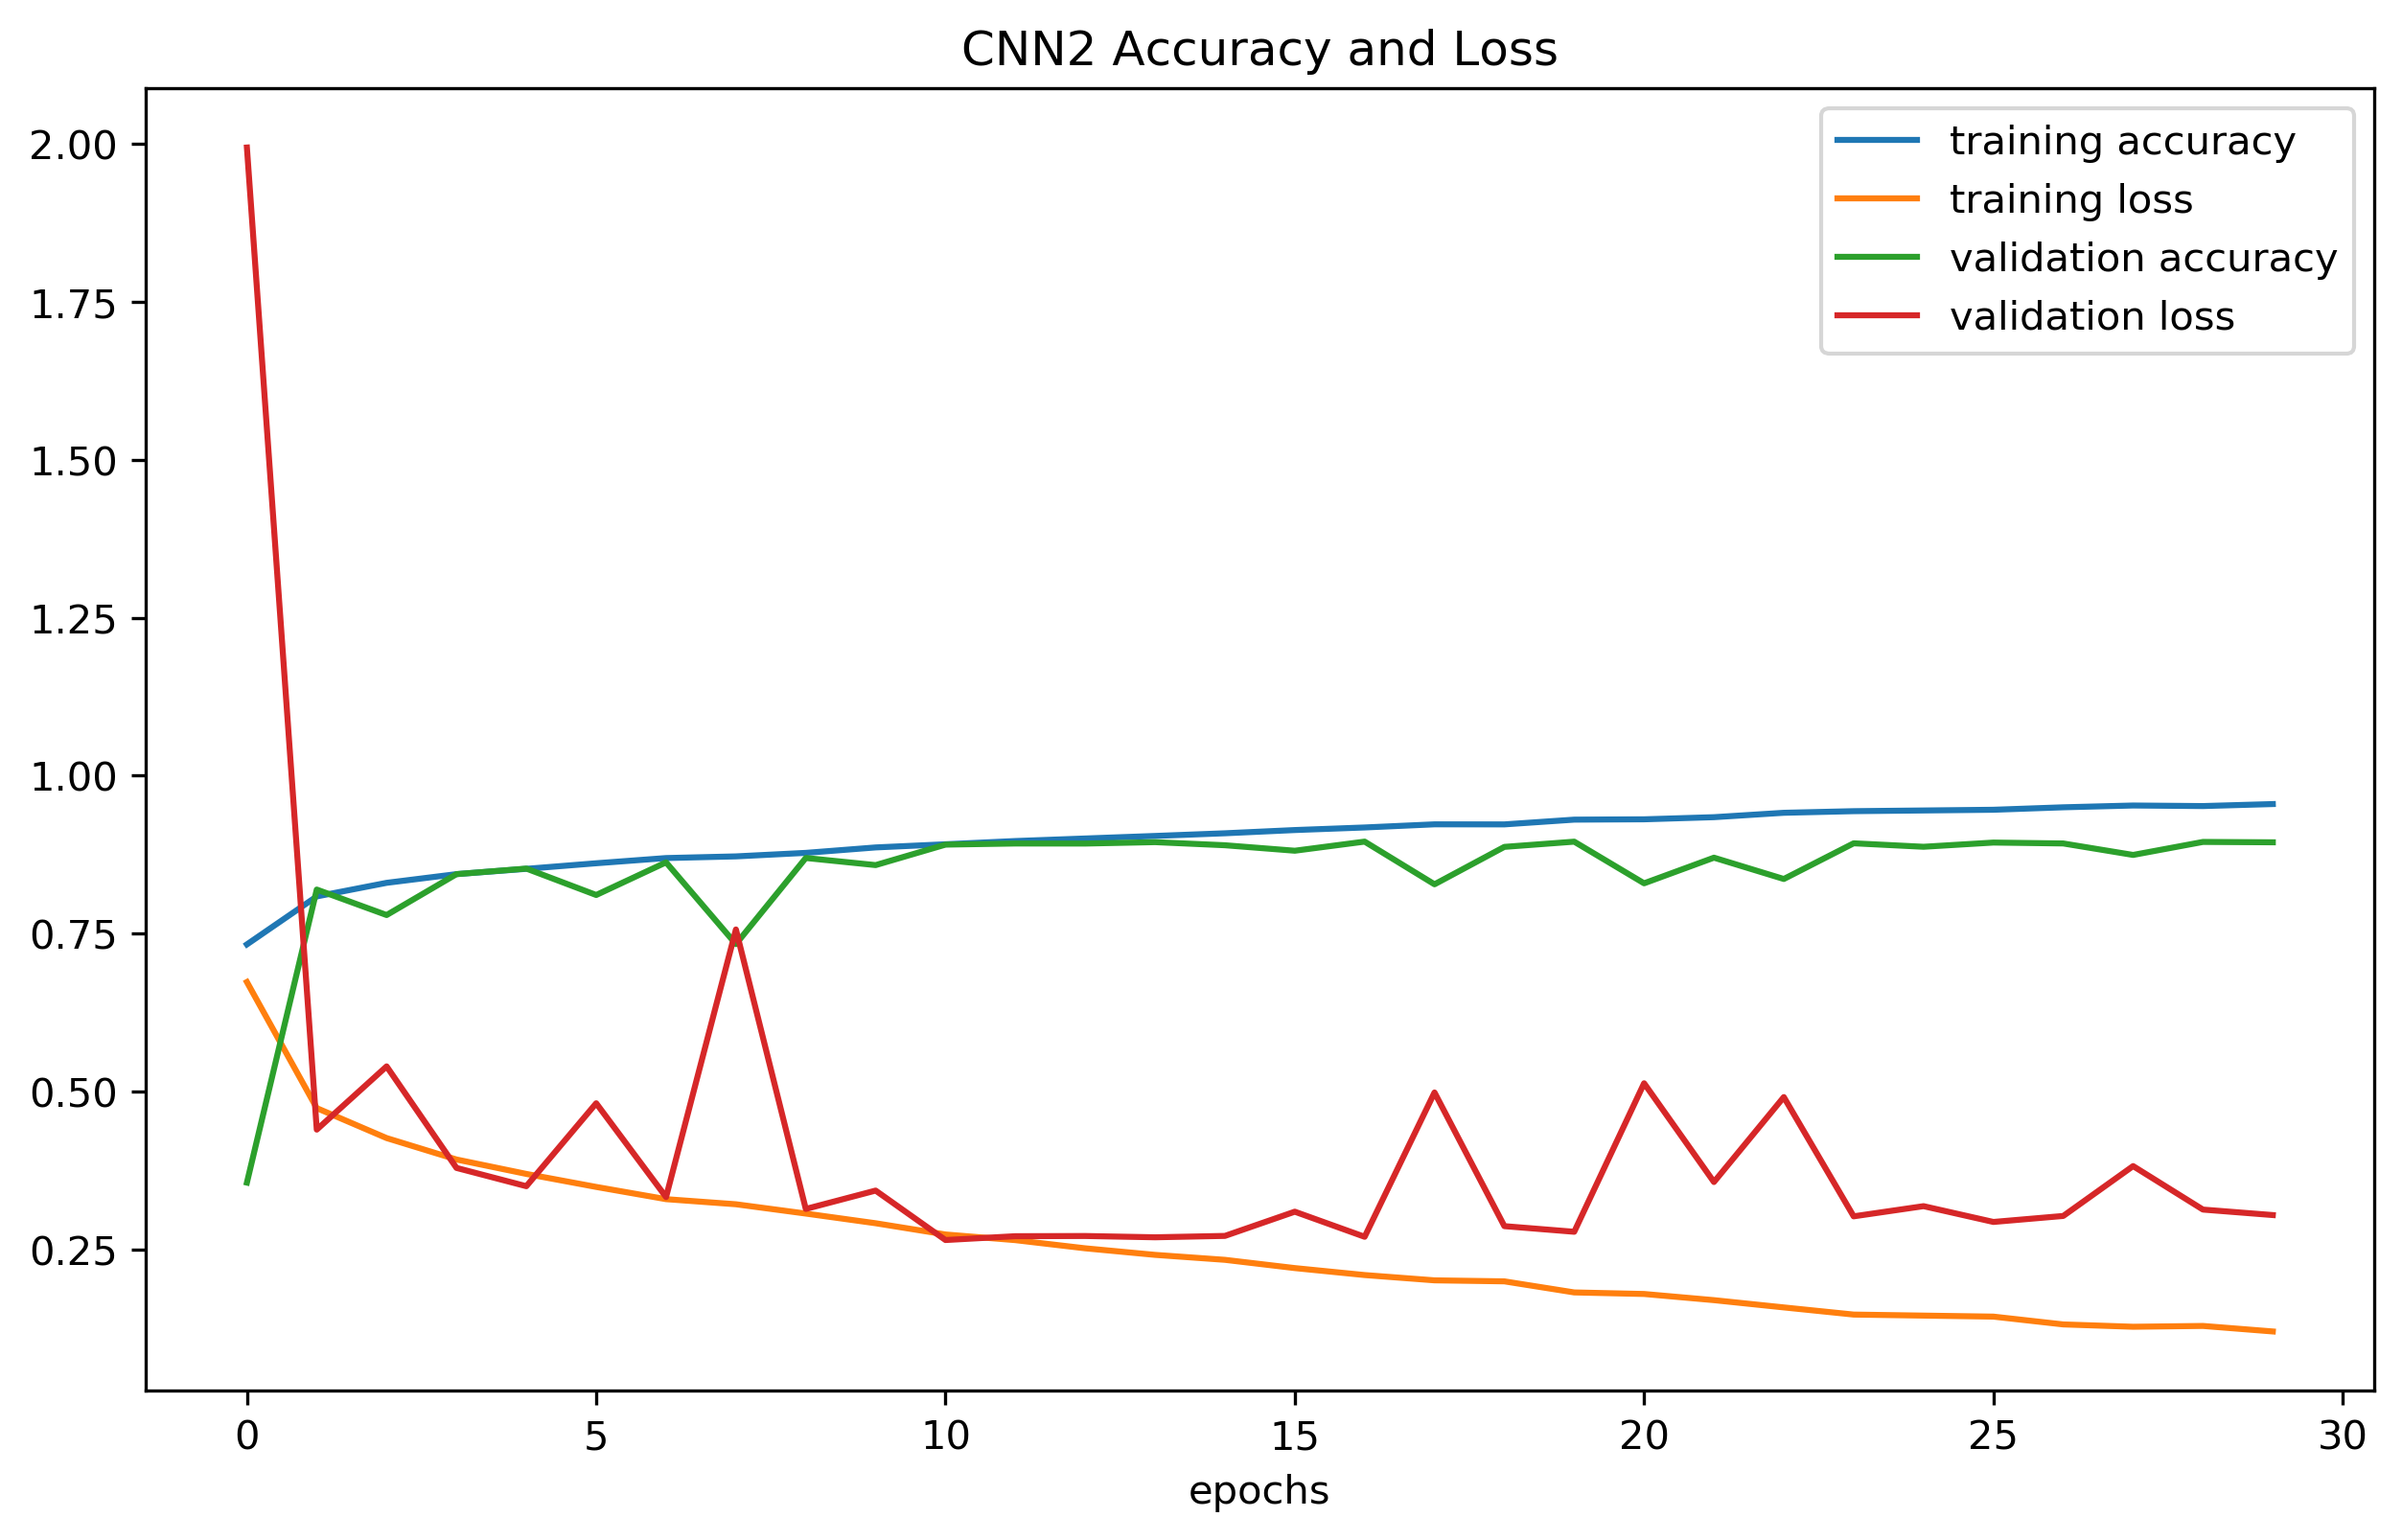
\includegraphics[width=0.8\textwidth]{./plots/CNN2_Result.png}
\end{center}
\end{figure}
% \vspace*{-1.5cm}
\begin{figure}[H]
\begin{center}
    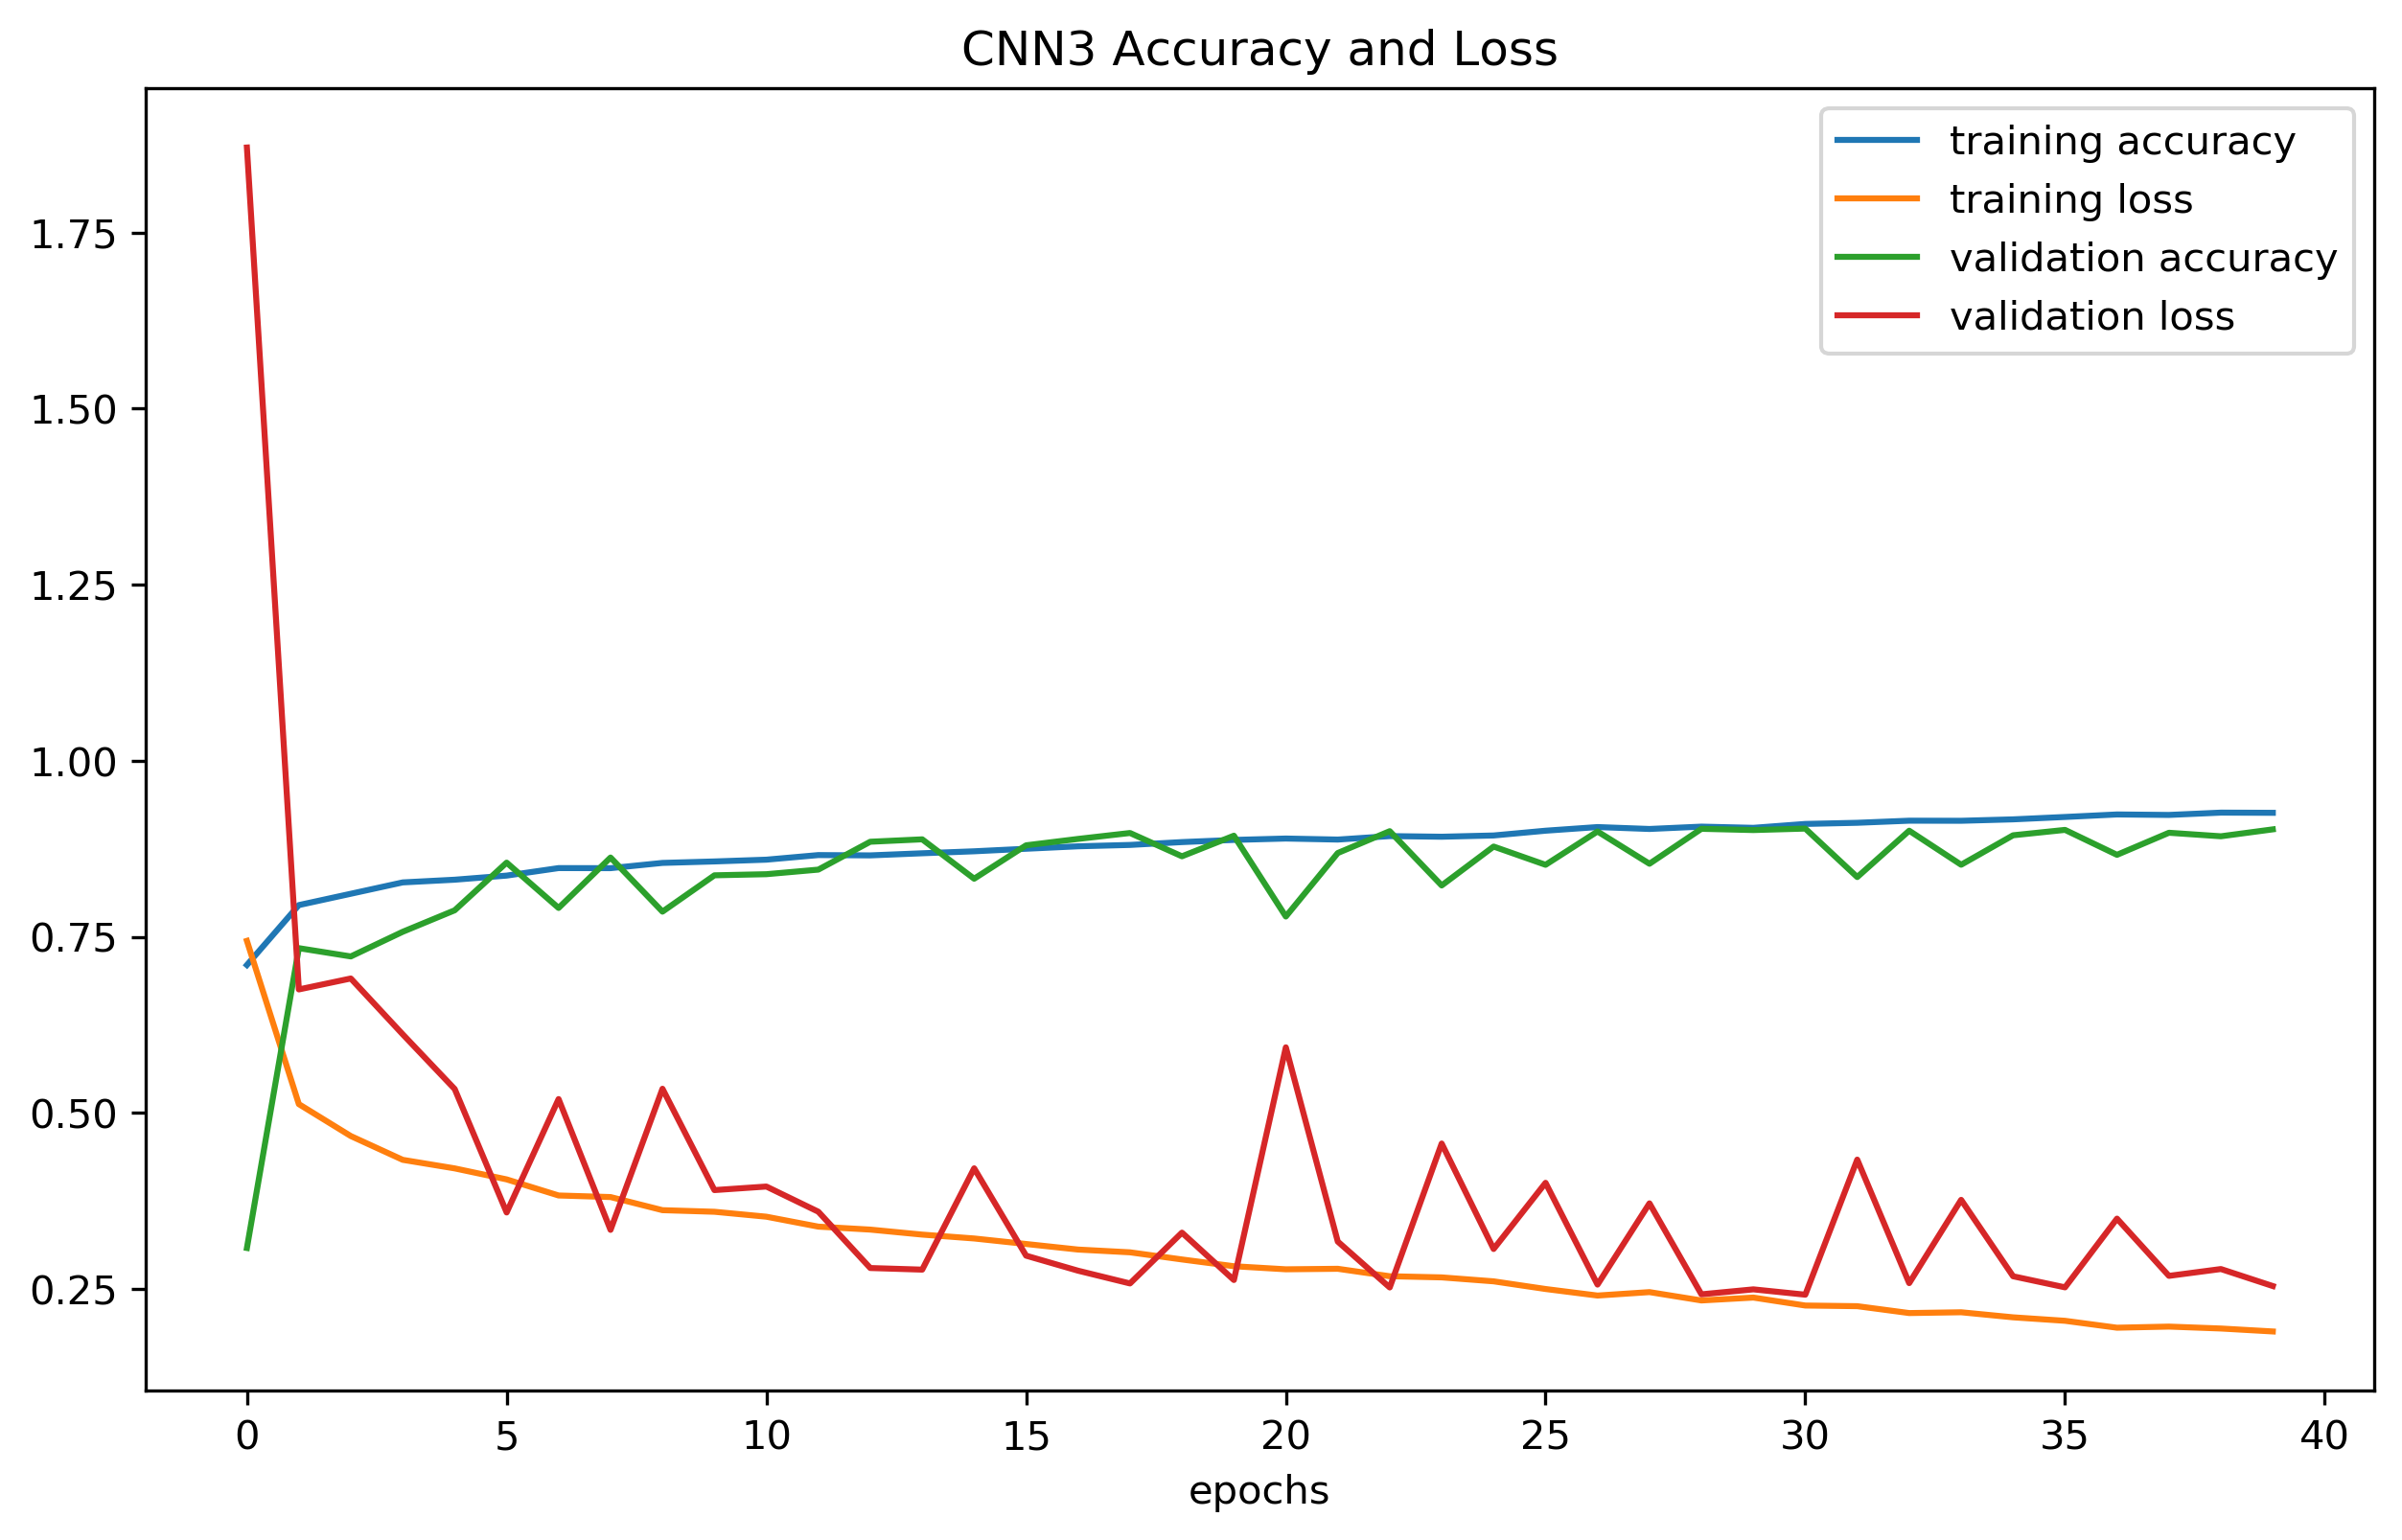
\includegraphics[width=0.8\textwidth]{./plots/CNN3_Result.png}
\end{center}
\end{figure}
% \vspace*{-1.5cm}
\begin{figure}[H]
\begin{center}
    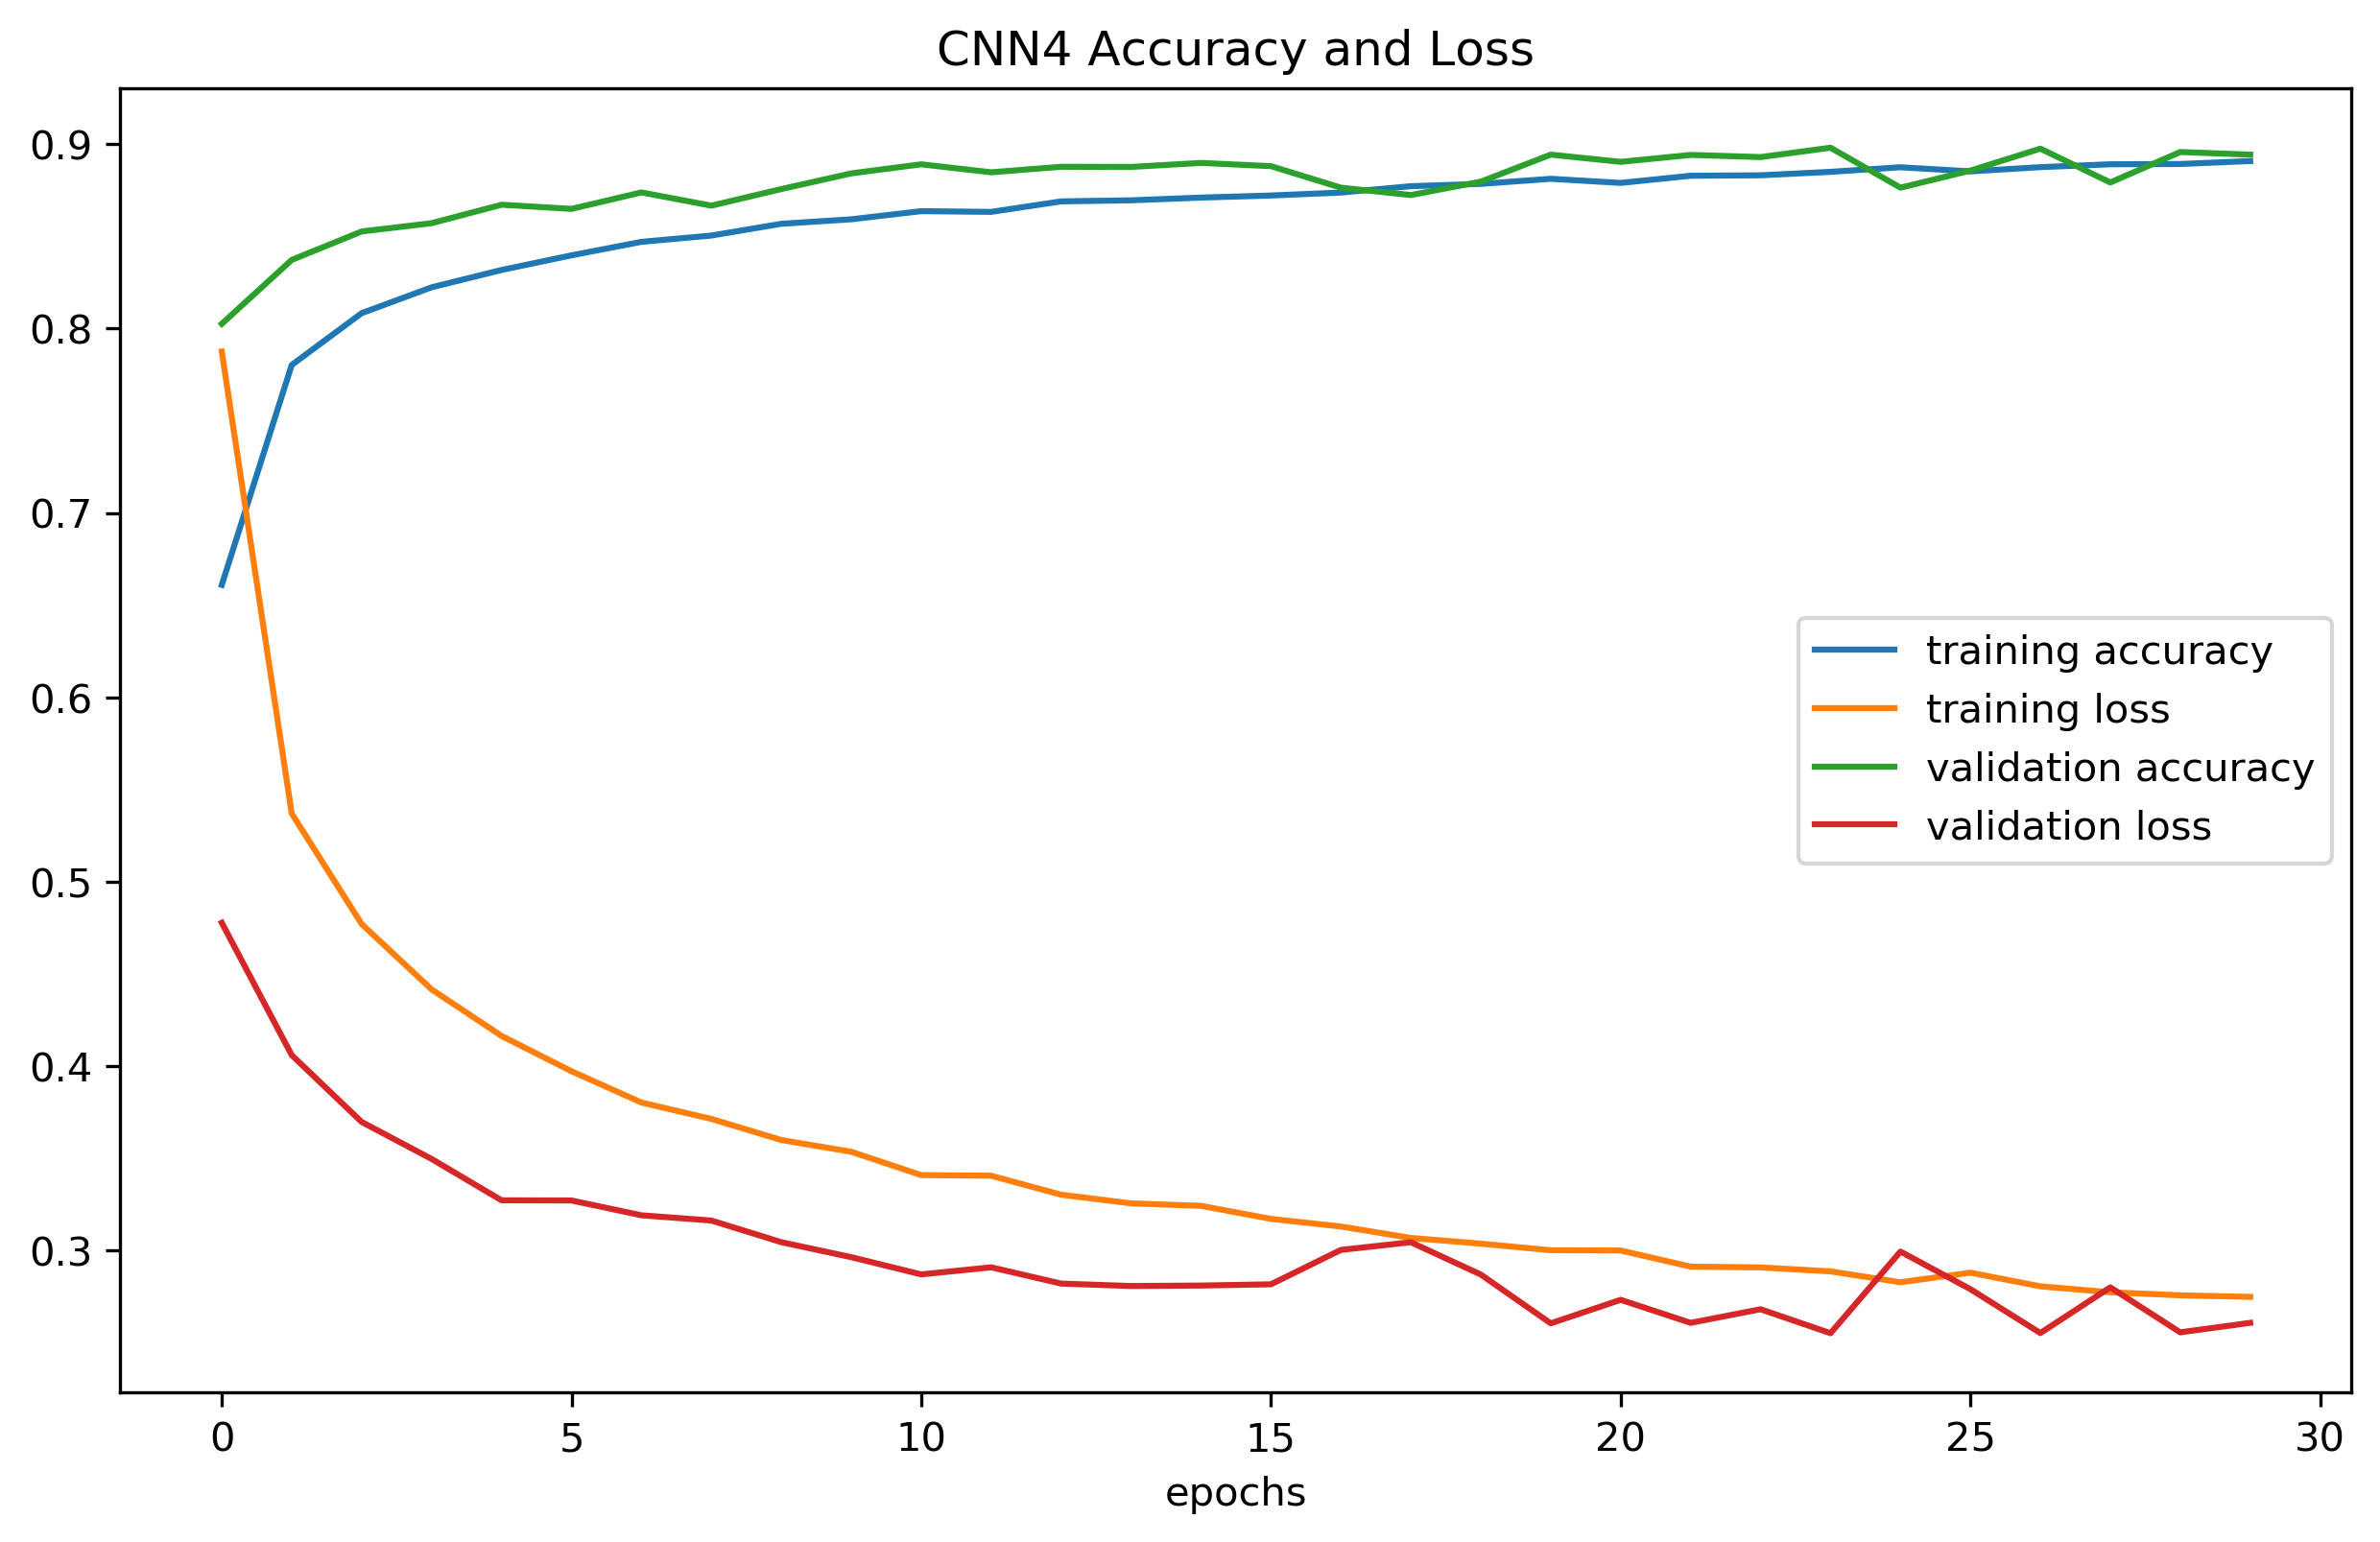
\includegraphics[width=0.8\textwidth]{./plots/CNN4_Result.png}
\end{center}
\end{figure}
% \vspace*{-1.5cm}
\begin{figure}[H]
\begin{center}
    \includegraphics[width=0.8\textwidth]{./plots/Resnet50_Result.png}
\end{center}
\end{figure}
\vspace*{-1.0cm}

Overall, the accuracy increases and the loss decreases for both training set and validation set as more epochs are presented to the model. The training accuracy and loss seem always monotonous. However, there are fluctuations with the validation accuracy and loss. E.g. in model 2 and 3 the validation accuracy dives to 0.8 and then bounces back to 0.9 from time to time. This may due to overfitting, a too large learning rate, not enough data points or some inadequate hyperparameters. And for Resnet50, the validation accuracy does not increase after the 4th epochs, which is definitely because of overfitting, and also the model is too big and it requires more training data. And from the above plots we learn that about 20 epochs is enough to train these models.

\subsubsection{Evaluate your code with other metrics on the training data and argue for the benefit of you approach.}
\end{document}